\documentclass[11pt,letterpaper]{article}
\usepackage[T1]{fontenc}
\usepackage[utf8]{inputenc}
\usepackage{lmodern}
\usepackage{microtype}
\usepackage[margin=1in]{geometry}
\usepackage{graphicx}
\usepackage{booktabs}
\usepackage{float}
\usepackage{longtable}
\usepackage{tabularx}
\usepackage{array}
\usepackage{multirow}
\usepackage{placeins}
\usepackage{pdflscape}
\usepackage{siunitx}
\usepackage{amsmath}
\usepackage[dvipsnames]{xcolor}
\usepackage{tikz}
\usetikzlibrary{positioning,arrows.meta,fit,calc}
\usepackage{caption}
\usepackage{subcaption}
\usepackage{enumitem}
\usepackage{newunicodechar}
\usepackage{fancyhdr}
\usepackage[backend=biber,style=numeric-comp,sorting=none,maxbibnames=4]{biblatex}
\addbibresource{references.bib}
\usepackage[colorlinks=true,linkcolor=MidnightBlue,citecolor=MidnightBlue,urlcolor=MidnightBlue]{hyperref}

\newunicodechar{µ}{\ensuremath{\mu}}
\newunicodechar{Ω}{\ensuremath{\Omega}}
\newunicodechar{±}{\ensuremath{\pm}}
\newunicodechar{×}{\ensuremath{\times}}
\newunicodechar{≈}{\ensuremath{\approx}}
\newunicodechar{−}{\ensuremath{-}}
\newunicodechar{°}{\ensuremath{^\circ}}

\sisetup{detect-all, per-mode=symbol, range-phrase=--, range-units=single}
\setlength{\parskip}{0.45em}
\setlength{\parindent}{0pt}
\captionsetup{font=small,labelfont=bf}
\renewcommand{\arraystretch}{1.15}
\newcolumntype{Y}{>{\raggedright\arraybackslash}X}
\newcolumntype{L}[1]{>{\raggedright\arraybackslash}p{#1}}

% ---------- placeholders ----------
\newcommand{\measured}{\fbox{\rule{0pt}{0.95em}\rule{2.0cm}{0pt}}}
\newcommand{\notesblank}{}
\newcommand{\todo}[1]{\par\noindent\fcolorbox{BurntOrange}{BurntOrange!7}{\parbox{\dimexpr\linewidth-2\fboxsep-2\fboxrule\relax}{\small\textbf{\textcolor{BurntOrange!80!black}{TODO (build notes):}} #1}}\par}
\newcommand{\est}{\textsuperscript{e}}
\newcommand{\simv}{\textsuperscript{s}}
\newcommand{\photo}[1]{\par\noindent\fbox{\parbox[c][5.5cm][c]{\dimexpr\linewidth-2\fboxsep-2\fboxrule\relax}{\centering\color{gray}\textit{Photo placeholder: #1}}}\par}

\pagestyle{fancy}
\fancyhf{}
\lhead{\small 40 m GaN class-E CW transmitter}
\rhead{\small NT7S, rev 7}
\cfoot{\small\thepage}

\title{A High-Efficiency 5\,W 40\,m GaN Class-E CW Transmitter\\for the 2027 FDIM QRP Transmitter Efficiency Challenge\\[0.4em]\large Design justification, simulation, build plan and test plan (rev 7)}
\author{Jason Milldrum, NT7S\\Etherkit}
\date{November 2026}

\begin{document}
\maketitle
\thispagestyle{empty}

\begin{abstract}
\noindent This report documents the rev 7 design of a crystal-controlled 40\,m CW transmitter built for the 2027 FDIM QRP Transmitter Efficiency Challenge, which scores DC-to-RF efficiency of the whole transmitter at \SI{12.0}{\volt} and 4--6\,W into \SI{50}{\ohm}. The power stage is a single-ended class-E amplifier using an EPC2036 eGaN FET, designed with Sokal's equations and followed by a 3-pole elliptic low-pass filter. A discrete Pierce oscillator, a 5\,V Schmitt buffer as gate driver, a high-side PMOS keying switch and a TPS62175 buck converter complete the transmitter. In ngspice the PA with its filter delivers \SI{5.10}{\watt} at \SI{96.4}{\percent} drain efficiency, and the estimated whole-transmitter efficiency is \SI{95.6}{\percent}. Every table pairs calculated or simulated values with blank columns for bench results, and the build and measurement sections are written as a plan to be filled in. Rev 6 added probe test points with adjacent ground pads and an unfitted gate-clamp footprint; a simulation of gate resistors and clamps shows neither is needed with this driver. Rev 7 replaces the supply terminal block and key header with a DC barrel jack and a 3.5\,mm key jack, and specifies a Molex 0731000105 right-angle BNC for J2 so every connector is a DigiKey part.
\end{abstract}

\medskip
\noindent\textbf{Revision numbering.} Prototype revisions are numbered; letters, starting from A, are reserved for released boards. The earlier prototype letters map to numerals as in Table~\ref{tab:revhist}. Historical file names keep their letters (for example \texttt{gen\_revE.py}); the project \texttt{README.md} maps each file to its numeral.

\begin{table}[H]\centering\small
\caption{Revision history. Prototype revisions 1--6 were labelled A--F \cite{projkicad,projnotes}.}\label{tab:revhist}
\begin{tabularx}{\textwidth}{@{}llY@{}}
\toprule Rev & Was & Change \\ \midrule
1 & A & Class-E PA stage with tank and L-match, no LPF \\
2 & B & 3-pole elliptic LPF added \\
3 & C & Discrete Pierce oscillator replaces the external drive input; PMOS keying of the PA rail (OpenBeacon~2); trap junctions moved clear of L3 \\
4 & D & Q3 and R4 removed so the key shorts R3 to ground; optional R12 shunt with TP1/TP2 and JP1 bypass; trimmable oscillator (C9) \\
5 & E & SMT parts wherever possible; TPS62175 buck with ferrite-bead filters; footprints and MPNs for every part \\
6 & F & Probe test points TP4--TP15 with adjacent ground pads; DNP gate-clamp footprint D1; gate R1 and clamp study \\
7 & -- & J1 DC barrel jack (Same Sky PJ-102AH) and J4 3.5\,mm key jack (SJ1-3523N) replace the terminal block and header \\
7 & -- & J2 RF output changed to Molex 0731000105 (DigiKey WM5524-ND) from Amphenol B6252HB-NPP3G-50, which DigiKey does not carry \\
\bottomrule
\end{tabularx}
\end{table}

\noindent\textbf{Conventions.} Values marked \est{} are estimates from hand calculation or published curves; values marked \simv{} are ngspice results. Neither is a measurement. Boxes \measured{} and orange \textsc{todo} panels are placeholders for bench data and build notes.

\tableofcontents
\clearpage

%=====================================================================
\section{Introduction and contest rules}\label{sec:intro}

The 2027 FDIM QRP Transmitter Efficiency Challenge was announced on the QRP ARCI mailing list on 18 November 2026 \cite{qrparci9611}. The announcement asks for a transmitter that, operated from a fixed \SI{12.0}{\volt} supply, delivers between \SI{4.0}{\watt} and \SI{6.0}{\watt} of RF in the 40\,m band into a \SI{50}{\ohm} load, using a 40\,m crystal as the frequency source \cite{qrparci9611}. Table~\ref{tab:rules} summarizes the rules as read from that message.

\begin{table}[h]
\centering\small
\caption{Contest rules as stated in qrparci message 9611 \cite{qrparci9611}, with the 2026 comparison from \cite{fdim2026rules}.}\label{tab:rules}
\begin{tabularx}{\textwidth}{@{}L{3.6cm}Y@{}}
\toprule
Item & Rule \\ \midrule
Supply & Fixed \SI{12.0}{\volt} supply \\
Output & \SIrange{4.0}{6.0}{\watt} RF in the 40\,m band into \SI{50}{\ohm} \\
Frequency source & A 40\,m crystal \\
Score & DC-to-RF efficiency: RF power into the dummy load divided by power drawn from the \SI{12.0}{\volt} supply \\
What counts & All circuit power (oscillator, driver, keying, fans). No other power source and no energy storage \\
Freedom & Any circuit, devices or amplifier class, provided a 40\,m crystal sets the frequency \\
Dates & Check-in by 8:30\,PM Friday May 21 at FDIM Club Night; awards dinner May 22 \\
Deliverable & Schematic for review and possible publication in \emph{QRP Quarterly} \\
Change from 2026 & The 2026 rules listed a 40\,m low-pass filter among the items provided at the event \cite{fdim2026rules}; the 2027 text lists only the supply, dummy load and power meter \\
\bottomrule
\end{tabularx}
\end{table}

The 2026 winner, Mark Frost AC9VC, reached \SI{86.0}{\percent} whole-transmitter efficiency with a GaN PA \cite{fdim2026winner}. Because that entry already used GaN, beating it means cutting losses in the passives and in the fixed overhead (oscillator, driver, keying, regulator), not only changing the transistor \cite{projnotes}. That observation drives most of the choices in Section~\ref{sec:just}.

%=====================================================================
\section{Architecture overview}\label{sec:arch}

Figure~\ref{fig:block} shows the signal and power paths of rev 7 (the rev 5 circuit plus test points and connector changes); the full schematic is in Figure~\ref{fig:sch} and Appendix~\ref{app:sch}. A discrete Pierce oscillator (Q4, Y1) runs continuously from a \SI{5}{\volt} buck converter (U2). Its output is AC-coupled into a 74LVC1G17 Schmitt buffer (U1), which drives the EPC2036 gate through R1. The \SI{12.0}{\volt} input passes an optional \SI{10}{\milli\ohm} Kelvin shunt (R12, or solder jumper JP1) and is keyed onto the PA rail by a P-channel MOSFET (Q2) controlled by a Morse key on J4. The class-E stage (L1 choke, C1 shunt, C2--L2 series tank with the L-match folded into L2, C3 shunt) feeds a 3-pole elliptic low-pass filter (C16, L3 with trap C17+C18, C19) and the BNC output J2 \cite{projkicad,projnotes}.

\begin{figure}[h]
\centering
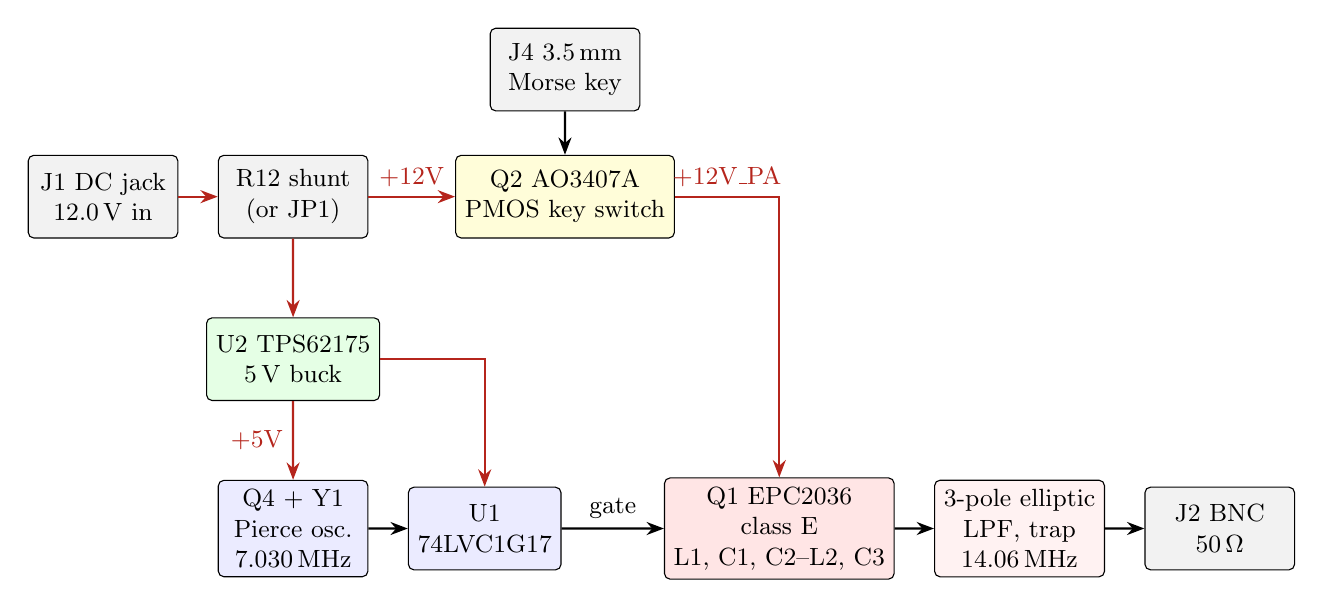
\begin{tikzpicture}[
  font=\small, scale=0.97,
  blk/.style={draw, rounded corners=2pt, align=center, minimum height=1.05cm, minimum width=1.9cm, fill=#1},
  blk/.default=white,
  arr/.style={-{Stealth[length=2.2mm]}, thick},
  pwr/.style={-{Stealth[length=2.2mm]}, thick, BrickRed},
  node distance=0.55cm and 0.5cm]
\node[blk=gray!10] (j1) {J1 DC jack\\\SI{12.0}{\volt} in};
\node[blk=gray!10, right=of j1] (sh) {R12 shunt\\(or JP1)};
\node[blk=yellow!15, right=1.1cm of sh] (q2) {Q2 AO3407A\\PMOS key switch};
\node[blk=gray!10, above=of q2] (j4) {J4 3.5\,mm\\Morse key};
\node[blk=green!10, below=1.0cm of sh] (u2) {U2 TPS62175\\\SI{5}{\volt} buck};
\node[blk=blue!8, below=1.0cm of u2] (osc) {Q4 + Y1\\Pierce osc.\\\SI{7.030}{\mega\hertz}};
\node[blk=blue!8, right=of osc] (u1) {U1\\74LVC1G17};
\node[blk=red!10, right=1.3cm of u1, minimum width=2.3cm] (pa) {Q1 EPC2036\\class E\\L1, C1, C2--L2, C3};
\node[blk=red!5, right=of pa] (lpf) {3-pole elliptic\\LPF, trap\\\SI{14.06}{\mega\hertz}};
\node[blk=gray!10, right=of lpf] (j2) {J2 BNC\\\SI{50}{\ohm}};
\draw[pwr] (j1) -- (sh);
\draw[pwr] (sh) -- node[above]{+12V} (q2);
\draw[arr] (j4) -- (q2);
\draw[pwr] (q2.east) -| node[pos=0.25,above]{+12V\_PA} (pa.north);
\draw[pwr] (sh) -- (u2);
\draw[pwr] (u2) -- node[left]{+5V} (osc);
\draw[pwr] (u2.east) -| (u1.north);
\draw[arr] (osc) -- (u1);
\draw[arr] (u1) -- node[above]{gate} (pa);
\draw[arr] (pa) -- (lpf);
\draw[arr] (lpf) -- (j2);
\end{tikzpicture}
\caption{Rev 7 block diagram (circuit unchanged from rev 5). Red arrows are DC power; black arrows are signal. Only the PA rail is keyed; the oscillator, U1 and U2 run continuously \cite{projkicad}.}\label{fig:block}
\end{figure}

Table~\ref{tab:keynums} collects the design point used throughout.

\begin{table}[h]
\centering\small
\caption{Design point and headline numbers. Sources: Sokal worked example \cite{sokal2001,projnotes} and ngspice runs \cite{projsim}.}\label{tab:keynums}
\begin{tabular}{@{}lll@{}}
\toprule
Quantity & Value & Basis \\ \midrule
Frequency, supply, target power & \SI{7.030}{\mega\hertz}, \SI{12.0}{\volt}, \SI{5.0}{\watt} & Design choice inside contest window \\
Loaded Q of the tank & 5 & Design choice \cite{projnotes} \\
Peak drain voltage & \SI{42.7}{\volt}\est{} / \SI{43.2}{\volt}\simv{} & Sokal eq.~3 ($3.56\,V_{DD}$) / trimmed run \\
DC current, PA rail & \SI{434}{\milli\ampere}\est{} / \SI{441}{\milli\ampere}\simv{} & Worked example / trimmed run \\
Output at J2 (trimmed, with LPF) & \SI{5.10}{\watt}\simv{} & \texttt{results\_v2.json} \\
Drain efficiency (with LPF) & \SI{96.4}{\percent}\simv{} & \texttt{results\_v2.json} \\
Whole-transmitter efficiency & \SI{95.6}{\percent}\est{} & Section~\ref{sec:budget} \\
\bottomrule
\end{tabular}
\end{table}

%=====================================================================
\section{Design justifications}\label{sec:just}

\subsection{Class E versus the alternatives}\label{sec:classE}

The contest is CW at one fixed supply voltage, so supply-modulation schemes such as envelope elimination and restoration give nothing \cite{projnotes}. Table~\ref{tab:published} lists published efficiencies that framed the choice. Single-ended class E is the simplest topology that reaches the high 80s to mid 90s in percent at HF: it switches at zero voltage, so the output capacitance of the switch is absorbed into the shunt capacitor rather than dumped every cycle \cite{sokal2001}. Its costs are a peak drain voltage of about $3.56\,V_{DD}$, sensitivity to load and tuning, and a strong second harmonic (about \SI{-20}{dBc} before filtering at $Q_L=5.1$) \cite{sokal2001}.

\begin{table}[h]
\centering\small
\caption{Published efficiencies, as each source states them \cite{projnotes}. Drain efficiency excludes the driver and oscillator; the contest scores the whole transmitter.}\label{tab:published}
\begin{tabularx}{\textwidth}{@{}L{3.1cm}L{2.4cm}YL{2.6cm}@{}}
\toprule
Topology & Devices & Published efficiency & Source \\ \midrule
Class E, single-ended & GaN FET & \SI{86.0}{\percent} whole transmitter, 40\,m, 4--6\,W, \SI{12.0}{\volt} & \cite{fdim2026winner} \\
Class E & 3$\times$ BS170 & About \SI{86}{\percent} at \SI{4.6}{\watt} from \SI{11.5}{\volt} (designer's claim) & \cite{sovina} \\
Class E & 2N7000 / BS170 & \SI{88}{\percent} at \SI{2}{\watt}, 40\,m, PA only & \cite{tayloe} \\
Class C drifting into E (W7EL) & D42C9 BJT & \SI{85}{\percent} collector or better, 7--9\,W, \SI{7}{\mega\hertz}; \SI{65}{\volt} peak measured & \cite[pp.~2.36, 2.37, 2.40]{emrfd} \\
Push-pull switching (QMX+ PA) & 2+2 BS170 & \SI{92}{\percent} on 40\,m at \SI{4.4}{\watt} with receive current subtracted & \cite{qrplabsqmx} \\
Class $\Phi_2$ (EF2) & MOSFET & Above \SI{92}{\percent} drain, over \SI{500}{\watt} at \SI{30}{\mega\hertz} & \cite{rivas2007} \\
Differential class E & EPC2037 & Driven from logic; gate drive \SI{13}{\milli\watt} at \SI{6.78}{\mega\hertz} & \cite[p.~3]{epcan021} \\
\bottomrule
\end{tabularx}
\end{table}

Alternatives considered and set aside \cite{projnotes}:
\begin{itemize}[nosep]
\item \textbf{Push-pull class E/F$_\text{odd}$} cancels even harmonics and allows a lighter filter, for an estimated 1--2 points over single-ended class E, but it needs two switches, two chokes, a tuned tank and an output transformer \cite{kee2003}. It is kept as a stretch path.
\item \textbf{Class $\Phi_2$ / EF2} lowers peak switch voltage to about $2V_{DD}$, which matters little at \SI{12}{\volt} because a \SI{100}{\volt} GaN part already has margin.
\item \textbf{Class E power oscillator} removes the separate oscillator and driver, but it stresses the crystal and risks the ``crystal as frequency source'' rule.
\item \textbf{IRF510 class E} is simple, but its gate drive is about \SI{584}{\milli\watt} at \SI{10}{\volt} and \SI{7}{\mega\hertz}\est, roughly 10\,\% of the input at 5\,W.
\end{itemize}

\subsection{Device choice: EPC2036, and Coss versus the shunt capacitor}\label{sec:device}

At \SI{5}{\watt} from \SI{12}{\volt} the drain current is only about \SI{0.43}{\ampere}, so a lower $R_{DS(on)}$ saves a few milliwatts while larger dies add gate charge and output capacitance whose losses scale with frequency \cite{projnotes}. The class-E shunt capacitance must total \SI{338.7}{\pico\farad} (Sokal eq.~8), and the device's $C_{oss}$ is part of it, so any part whose effective $C_{oss}$ exceeds that total cannot be used at all. Table~\ref{tab:devices} reproduces the device comparison. The loss model uses $1.365\,R_{DS(on)}$ for conduction (Sokal eq.~1), $Q_g V_g f$ for gate drive, Sokal eq.~2 for turn-off with assumed fall times, and a placeholder 10\,\% per cycle for $C_{oss}$ hysteresis \cite{sokal2001,projnotes}.

\begin{table}[h]
\centering\footnotesize\setlength{\tabcolsep}{2.6pt}
\caption{Candidate switches against the class-E budget (\SI{7.03}{\mega\hertz}, \SI{12.0}{\volt}, \SI{5}{\watt}, $Q_L=5$). Device data from datasheets \cite{epc2036ds,epcothers,otherdevices}; losses are estimates \cite{projnotes}.}\label{tab:devices}
\begin{tabular}{@{}lrrrrll@{}}
\toprule
Part & $V_{DS}$ & $R_{DS(on)}$ max & $C_{oss,\mathrm{eff}}$ & $Q_g$ & Loss\est{} (no hyst./hyst.) & Verdict \\ \midrule
EPC2036 & \SI{100}{\volt} & \SI{73}{\milli\ohm} & \SI{78}{\pico\farad} & \SI{0.70}{\nano\coulomb} & 66 / \SI{116}{\milli\watt} & Best estimate \\
EPC2051 & \SI{100}{\volt} & \SI{25}{\milli\ohm} & \SI{146}{\pico\farad} & \SI{1.8}{\nano\coulomb} & 80 / \SI{174}{\milli\watt} & Close second \\
EPC2012C & \SI{200}{\volt} & \SI{100}{\milli\ohm} & about \SI{130}{\pico\farad} & \SI{1.0}{\nano\coulomb} & 90 / \SI{173}{\milli\watt} & Voltage margin \\
EPC2037 & \SI{100}{\volt} & \SI{550}{\milli\ohm} & \SI{12}{\pico\farad} & \SI{0.115}{\nano\coulomb} & 283 / \SI{291}{\milli\watt} & Too resistive \\
GS61004B & \SI{100}{\volt} & \SI{22}{\milli\ohm} & \SI{180}{\pico\farad} & \SI{3.3}{\nano\coulomb} & 155 / \SI{270}{\milli\watt} & Easier to solder \\
EPC2045 & \SI{100}{\volt} & \SI{7}{\milli\ohm} & \SI{500}{\pico\farad} & \SI{6.0}{\nano\coulomb} & 219 / \SI{540}{\milli\watt} & $C_{oss}$ exceeds C1 \\
BSZ146N10LS5 (Si) & \SI{100}{\volt} & \SI{20.8}{\milli\ohm} & \SI{400}{\pico\farad} & \SI{7.6}{\nano\coulomb} & 269 / \SI{526}{\milli\watt} & $C_{oss}$ exceeds C1 \\
3$\times$ BS170 (Si) & \SI{60}{\volt} & about \SI{0.83}{\ohm}\est & \SI{75}{\pico\farad} & about \SI{0.9}{\nano\coulomb} & 560 / \SI{608}{\milli\watt} & Kit fallback \\
IRF510 (Si) & \SI{100}{\volt} & \SI{0.54}{\ohm} & \SI{81}{\pico\farad} & \SI{8.3}{\nano\coulomb} & 967 / \SI{1019}{\milli\watt} & Gate drive too costly \\
\bottomrule
\end{tabular}
\end{table}

EPC2036 has the lowest estimated loss and can be driven straight from a logic gate \cite{epcan021}. Paralleling two of them halves conduction loss to about \SI{18}{\milli\watt} but doubles gate drive and $C_{oss}$, for about \SI{72}{\milli\watt} against \SI{66}{\milli\watt}\est{} for one part, so there is no gain at 5\,W \cite{projnotes}. Its constraints are a \SI{6}{\volt} absolute-maximum gate, ESD sensitivity, no body diode (reverse conduction at about \SI{1.9}{\volt}), and a $0.9\times\SI{0.9}{\milli\meter}$ chip-scale package \cite{epc2036ds,lidow,epcrel6}. The worked example takes $C_{oss}\approx\SI{50}{\pico\farad}$ (typical at \SI{50}{\volt}) and puts C1 at about \SI{285}{\pico\farad}; the effective $C_{oss}$ of \SI{78}{\pico\farad} implies about \SI{261}{\pico\farad} ($338.7-78$), which the simulation confirms (Section~\ref{sec:c1trim}).

\subsection{Gate drive: 74LVC1G17 versus LMG1020}\label{sec:gate}

Every milliampere of driver current is scored, so the driver is chosen for its draw from \SI{12}{\volt} rather than for edge speed (Table~\ref{tab:drivers}). EPC's AN021 drove an EPC2037 class-E stage directly from logic \cite{epcan021}. A single 74LVC1G-class gate at \SI{5}{\volt} supplies the EPC2036's \SI{0.7}{\nano\coulomb} gate charge, and its Schmitt input gives a clean edge from the oscillator's sine-like swing \cite{tiLVC1G17}. The LMG1020 is a \SI{60}{\mega\hertz} GaN driver, but its \SI{40}{\milli\ampere} operating current at \SI{30}{\mega\hertz} scales to about \SI{170}{\milli\watt}\est{} here, which would cost about three efficiency points \cite{tiLMG1020,projnotes}.

\begin{table}[h]
\centering\small
\caption{Gate-driver options for EPC2036 at \SI{7.03}{\mega\hertz}; draws are estimates \cite{projnotes}.}\label{tab:drivers}
\begin{tabularx}{\textwidth}{@{}L{3.6cm}YL{2.6cm}L{2.4cm}@{}}
\toprule
Driver & Datasheet fact & Draw from 12\,V\est & Fit \\ \midrule
74LVC1G-class gate on a 5\,V buck (85\,\%) & AN021 drove EPC2037 from logic, \SI{13}{\milli\watt} gate drive at \SI{6.78}{\mega\hertz} \cite{epcan021} & about \SI{29}{\milli\watt} & Chosen \\
Same gate on a 5\,V LDO & LDO draws the same current at 12\,V & about \SI{59}{\milli\watt} & OK \\
UCC27611 & 4--18\,V supply, internal 5\,V regulator \cite{tiUCC27611} & about \SI{60}{\milli\watt} & For larger FETs \\
LMG1020 & \SI{40}{\milli\ampere} operating at \SI{30}{\mega\hertz}, \SI{0.1}{\pico\farad} load \cite{tiLMG1020} & about \SI{170}{\milli\watt} & Overkill \\
\bottomrule
\end{tabularx}
\end{table}

In simulation the gate swings from \SI{-0.04}{\volt} to \SI{5.00}{\volt} with an ideal driver and \SI{2}{\nano\henry} gate loop, inside the \SI{6}{\volt} rating, and the driver delivers \SI{16.6}{\milli\watt}\simv{}; $Q_g V f$ with the typical $Q_g$ gives \SI{24.6}{\milli\watt}\est, the difference being Miller charge avoided by zero-voltage switching \cite{projsim,projnotes}.

\subsubsection*{Gate-voltage mitigation: R1 and clamps (rev 6)}
The EPC2036 gate is rated \SI{6}{\volt} and \SI{-4}{\volt} absolute maximum, with \SI{75}{\pico\farad} typical input capacitance and up to \SI{0.9}{\milli\ampere} forward gate leakage at \SI{5}{\volt} \cite{epc2036ds}. Two common mitigations, a series gate resistor and a gate-source clamp, were simulated in Section~\ref{sec:gatesim}. The 74LVC1G17 output resistance is at most about \SI{22}{\ohm} at \SI{4.5}{\volt} (from $V_{OH}\ge\SI{3.8}{\volt}$ at \SI{-32}{\milli\ampere}) \cite{tiLVC1G17}, and the simulation assumes \SI{7}{\ohm}\est. With that source resistance the gate loop is overdamped up to about \SI{2}{\nano\henry}: there is no overshoot, and every ohm of R1 only costs efficiency, at most 0.065 points for \SI{10}{\ohm}. Even a \SI{5}{\nano\henry} stress loop peaks at \SI{5.38}{\volt}, and \SI{2.2}{\ohm} brings that to \SI{5.08}{\volt} \cite{projsim}. A zener clamp costs 0.12 to 0.14 points in simulation, and the datasheet capacitance suggests more (Section~\ref{sec:gatesim}). A BZX84C6V2 cannot hold the gate under \SI{6}{\volt}: its datasheet $V_Z$ is 5.8--\SI{6.6}{\volt} at \SI{5}{\milli\ampere} \cite{onsemiBZX84}. A BZX84C5V6 can start conducting at a \SI{5}{\volt} gate ($V_Z$ as low as \SI{4.8}{\volt} at \SI{1}{\milli\ampere}).

\textbf{Decision for rev 6, kept in rev 7:} R1 stays \SI{0}{\ohm}, with a 0603 footprint. Fit \SI{2.2}{\ohm} only if TP4/TP5 shows more than about \SI{5.5}{\volt}. D1 is a do-not-populate (DNP) SOT-23 footprint (K to gate, A to source), which takes either a BAT54-type Schottky or a BZX84 zener, since both use SOT-23 pin 1 for the anode and pin 3 for the cathode \cite{onsemiBAT54,onsemiBZX84}. It stays unfitted unless measurement shows a real problem.

\subsection{Class-E design equations and component values}\label{sec:sokal}

The load network follows Sokal's design equations \cite{sokal2001}. The load resistance for output $P$ at supply $V$ and loaded Q is
\begin{equation*}
R = \frac{V^2}{P}\cdot 0.576801\left(1.0000086-\frac{0.414395}{Q_L}-\frac{0.577501}{Q_L^2}+\frac{0.205967}{Q_L^3}\right) \tag{Sokal 6a}
\end{equation*}
and the efficiency including series losses and a finite fall time is
\begin{equation*}
\eta = \frac{R_{load}}{R_{load}+ESR_{L2}+ESR_{C2}+1.365R_{on}+0.2116\,ESR_{C1}} - \frac{(2\pi A)^2}{12} - 0.01. \tag{Sokal 2}
\end{equation*}
At $Q_L=5$ the fit of eq.~6a gives 0.51663 against 0.51659 in Sokal's Table~I \cite{projnotes}. The inputs are \SI{12.0}{\volt}, \SI{5.0}{\watt} at the load network, $Q_L=5$, $R_{on}=\SI{73}{\milli\ohm}$, with assumed L2 $Q_u=250$, C0G ESR \SI{0.02}{\ohm} and a \SI{3}{\nano\second} fall time \cite{projnotes}. Table~\ref{tab:sokal} lists the results and the built values.

\begin{table}[h]
\centering\small
\caption{Worked class-E example at \SI{7.030}{\mega\hertz} \cite{sokal2001,projnotes} and the values on the rev 7 schematic \cite{projkicad}.}\label{tab:sokal}
\begin{tabularx}{\textwidth}{@{}L{4.3cm}L{4.4cm}Y@{}}
\toprule
Quantity & Calculated & Built (rev 7) \\ \midrule
$R$ (eq.~6a) & \SI{14.27}{\ohm}, sized for \SI{5.21}{\watt} & -- \\
$R_{load}$ after losses (eq.~1) & \SI{13.87}{\ohm} & L-match to \SI{50}{\ohm} \\
Drain efficiency (eq.~2) & \SI{95.9}{\percent}\est & -- \\
C1 shunt (eq.~8) & \SI{338.7}{\pico\farad} total incl.\ $C_{oss}$, about \SI{285}{\pico\farad} external & 270 + \SI{15}{\pico\farad} = \SI{285}{\pico\farad}; optimum about \SI{260}{\pico\farad}\simv \\
C2 series (eq.~9) & \SI{424.5}{\pico\farad} & 390 + \SI{33}{\pico\farad} = \SI{423}{\pico\farad}, \SI{200}{\volt} C0G \\
L2 (eq.~10) & \SI{1.616}{\micro\henry} & -- \\
L-match \SI{13.87}{\ohm} to \SI{50}{\ohm} & $Q=1.61$: \SI{0.507}{\micro\henry} series, \SI{731}{\pico\farad} shunt & C3 = 680 + \SI{51}{\pico\farad} = \SI{731}{\pico\farad} \\
L2 incl.\ match series arm & \SI{2.122}{\micro\henry} & T-80-6, 22\,t \#16: \SI{2.18}{\micro\henry} \\
L1 DC feed & $\geq$\SI{46.3}{\micro\henry} ($X_{L1}\geq 30X_{C1}$) & FT-50-61, 26\,t \#24, about \SI{47}{\micro\henry} \\
DC current & \SI{434}{\milli\ampere} & -- \\
Peak drain voltage & \SI{42.7}{\volt} ($3.56V_{DD}$, eq.~3) & EPC2036 rated \SI{100}{\volt} \\
Peak drain current & about \SI{1.24}{\ampere} ($2.86\,I_{dc}$, ideal analysis) & -- \\
2nd harmonic before filtering & \SI{-20}{dBc} at $Q_L=5.1$ & LPF needs $\geq$\SI{23}{\decibel} at 14\,MHz \\
\bottomrule
\end{tabularx}
\end{table}

C2 sees about \SI{58}{\volt} peak (\SI{12}{\volt} DC plus about \SI{46}{\volt} RF)\est, so it uses \SI{200}{\volt} C0G parts; C1, C3 and the filter capacitors are \SI{100}{\volt} C0G \cite{projkicad}. Odd values are made from standard-value pairs (Table~\ref{tab:bom}).

\paragraph{C1 trim to about 260 pF.}\label{sec:c1trim}
Table~\ref{tab:c1sweep} sweeps C1 and L2 in ngspice without the filter. With L2 as wound (\SI{2.18}{\micro\henry}) the stage makes \SI{4.06}{\watt}, not 5\,W: each extra \SI{58}{\nano\henry} (\SI{2.6}{\ohm} at \SI{7.03}{\mega\hertz}) costs about \SI{0.8}{\watt} because the tank's excess reactance sets the output. At the design value of \SI{2.122}{\micro\henry} with C1 = \SI{260}{\pico\farad} the result is \SI{5.03}{\watt}, \SI{433}{\milli\ampere} and \SI{43.1}{\volt} peak, close to the hand calculation \cite{projsim,projnotes}. Turn-on voltage is lowest near \SI{260}{\pico\farad}, which matches $338.7-78\approx\SI{261}{\pico\farad}$. The build therefore trims L2 toward \SI{2.122}{\micro\henry} and C1 toward \SI{260}{\pico\farad} on the bench (Section~\ref{sec:trim}).

\begin{table}[h]
\centering\small
\caption{Simulated C1/L2 sweep, no LPF, \SI{50}{\ohm} load \cite{projsim}.}\label{tab:c1sweep}
\begin{tabular}{@{}llrrrrr@{}}
\toprule
C1 & L2 & Output & Drain eff. & Peak drain & $v_D$ at turn-on & 2nd harm. \\ \midrule
\SI{260}{\pico\farad} & \SI{2.18}{\micro\henry} & \SI{4.21}{\watt} & \SI{96.9}{\percent} & \SI{42.3}{\volt} & \SI{0.06}{\volt} & \SI{-26.6}{dBc} \\
\SI{285}{\pico\farad} & \SI{2.18}{\micro\henry} & \SI{4.06}{\watt} & \SI{96.8}{\percent} & \SI{40.7}{\volt} & \SI{2.0}{\volt} & \SI{-27.1}{dBc} \\
\SI{310}{\pico\farad} & \SI{2.18}{\micro\henry} & \SI{3.94}{\watt} & \SI{96.5}{\percent} & \SI{39.3}{\volt} & \SI{3.9}{\volt} & \SI{-27.7}{dBc} \\
\SI{260}{\pico\farad} & \SI{2.122}{\micro\henry} & \SI{5.03}{\watt} & \SI{96.8}{\percent} & \SI{43.1}{\volt} & \SI{0.7}{\volt} & \SI{-26.8}{dBc} \\
\SI{285}{\pico\farad} & \SI{2.122}{\micro\henry} & \SI{4.86}{\watt} & \SI{96.8}{\percent} & \SI{41.4}{\volt} & \SI{2.3}{\volt} & \SI{-27.4}{dBc} \\
\SI{310}{\pico\farad} & \SI{2.122}{\micro\henry} & \SI{4.71}{\watt} & \SI{96.5}{\percent} & \SI{40.0}{\volt} & \SI{3.9}{\volt} & \SI{-27.9}{dBc} \\
\bottomrule
\end{tabular}
\end{table}

\subsection{Inductor cores: mix 6 versus mix 2, T-80 versus T-106}\label{sec:cores}

The tank current is set by the load: $I=\sqrt{2\times\SI{5.212}{\watt}/\SI{14.27}{\ohm}}=\SI{0.855}{\ampere}$ peak. At \SI{2.12}{\micro\henry} the reactance is \SI{93.7}{\ohm}, so the inductor circulates $I^2X = \SI{34.2}{var}$ and dissipates $P = \SI{34.2}{\watt}/Q_u$ \cite{projnotes}. Inductor $Q_u$ therefore converts directly into watts. Table~\ref{tab:qdata} lists the published Q data found; no published Q exists for these exact windings at \SI{7.03}{\mega\hertz}, so the $Q_u$ values in Table~\ref{tab:l2cores} are estimates from a wire-plus-core model calibrated to KN5L's measured T68-6 \cite{kn5l,projnotes}.

\begin{table}[h]
\centering\small
\caption{Published Q data used to calibrate the estimates \cite{micrometalsT80,kn5l,emrfd}.}\label{tab:qdata}
\begin{tabularx}{\textwidth}{@{}L{3.3cm}L{3.4cm}L{2.3cm}L{2.7cm}Y@{}}
\toprule
Source & Core and winding & Frequency & Q & Kind \\ \midrule
Micrometals T80-6 & 20\,t \#20 (about \SI{1.8}{\micro\henry}) & \SI{8}{\mega\hertz} & $\geq 270$ & Production minimum \\
Micrometals T68-6 & 23\,t \#20 & \SI{10}{\mega\hertz} & $\geq 266$ & Production minimum \\
Micrometals T50-6 & 25\,t \#22 & \SI{10}{\mega\hertz} & $\geq 237$ & Production minimum \\
KN5L bench & T68-6, 23\,t \#20 & 5/6/9/12\,MHz & 285/294/292/275 & Measured (VNA) \\
EMRFD Table 3A, p.~3.14 & T50-6, 20\,t, \SI{1.6}{\micro\henry} & \SI{7.05}{\mega\hertz} & 250 & Design $Q_u$ \\
EMRFD p.~7.36 & Air coil, 13\,t \#14, 3.5\,in form & \SI{7}{\mega\hertz} & 371 & Measured \\
\bottomrule
\end{tabularx}
\end{table}

\begin{table}[h]
\centering\small
\caption{Main inductor (\SI{2.12}{\micro\henry}) candidates; $Q_u$, loss and rise are estimates \cite{projnotes,micrometalsT80,amidon135}.}\label{tab:l2cores}
\begin{tabular}{@{}llrrrl@{}}
\toprule
Core & Turns, wire & $Q_u$\est & Loss at 5\,W\est & Peak flux & Verdict \\ \midrule
T-50-2 & 21\,t \#22 & about 250 & \SI{139}{\milli\watt} & 77\,G (over 57\,G) & Baseline \\
T-50-6 & 23\,t \#22 & about 250 & \SI{134}{\milli\watt} & 70\,G (over 57\,G) & Too small \\
T-68-6 & 21\,t \#20 & about 280 & \SI{121}{\milli\watt} & 48\,G & OK \\
T-80-2 & 20\,t \#16 & about 300 & \SI{113}{\milli\watt} & 39\,G & Good \\
T-80-6 & 22\,t \#16 & about 330 & \SI{104}{\milli\watt} & 36\,G & Built \\
T-106-2 & 13\,t \#14 & about 350 & \SI{97}{\milli\watt} & 21\,G & Good \\
T-106-6 & 14\,t \#14 & about 400 & \SI{85}{\milli\watt} & 20\,G & Best estimate \\
Air, 1\,in form, \#12 & 14\,t & about 350 & \SI{97}{\milli\watt} & no core & Needs clearance \\
\bottomrule
\end{tabular}
\end{table}

Mix 6 beats mix 2 at \SI{7}{\mega\hertz} on core loss and on temperature coefficient (\SI{+35}{ppm\per\celsius} against \SI{+95}{ppm\per\celsius}), and stepping up from T-50 brings the flux under Amidon's 57\,G guideline for \SI{7}{\mega\hertz} \cite{projnotes,amidon135}. T-106-6 is the lowest-loss estimate. The build uses T-80-6 for both L2 and L3 instead: one core type, a smaller footprint, and an estimated cost of \SI{18}{\milli\watt} (about 0.3 points) against T-106-6 in every position \cite{projnotes}. An air coil only matches T-80-6 at \#12 on a 1\,in form, with added clearance and layout sensitivity; toroids keep the field in the core and can sit near a ground plane \cite[p.~3.32]{emrfd}. L2 is wound with \#16 (\SI{50.8}{mil}, about \SI{1.29}{\milli\meter} bare) \cite[Table 22.44, p.~22.39]{arrl2023}.

\subsection{Drain choke: FT-50-61, not mix 43}\label{sec:choke}

The choke sits across the drain's RF voltage (a \SI{19.7}{\volt} peak fundamental plus \SI{10.2}{\volt} at $2f$ for the ideal class-E waveform\est), so its parallel loss resistance $R_p$ dissipates real power, $P\approx V^2/2R_p$ \cite{projnotes}. Fair-Rite's complex-permeability data at \SI{7.03}{\mega\hertz} gives 43 material a material Q of about 1.4 ($\mu'\approx327$, $\mu''\approx228$), while 61 material is nearly lossless there \cite{fairrite43,projnotes}. With 43, fewer turns means more loss; with 61, core loss is negligible. Table~\ref{tab:choke} compares the candidates. FT-50-61 with 26\,t \#24 (about \SI{47}{\micro\henry} at $A_L=69$\,nH/t$^2$ $\pm$25\,\%) dissipates about \SI{8}{\milli\watt} against the \SI{52}{\milli\watt} allowance in the loss budget, saving about 0.7 points\est{} \cite{fairrite61,projnotes}. Since C2 blocks DC, L2 carries only RF; the \SI{434}{\milli\ampere} DC flows in L1, which at \SI{4.8}{Oe} is far from saturation in 61 material.

\begin{table}[h]
\centering\small
\caption{Drain-choke candidates at \SI{12.0}{\volt}, \SI{434}{\milli\ampere}, \SI{7.03}{\mega\hertz}. Losses are estimates from Fair-Rite permeability data \cite{projnotes,fairrite43,fairrite61}.}\label{tab:choke}
\begin{tabular}{@{}llrrrrl@{}}
\toprule
Core & Turns & $L$ & $|Z|$ / $R_p$ & Core loss & Cu loss & Verdict \\ \midrule
FT-50-43 & 20\,t \#26 & \SI{176}{\micro\henry} & 3.87\,k / \SI{6.8}{\kilo\ohm} & \SI{36}{\milli\watt} & \SI{9}{\milli\watt} & Bias roll-off likely \\
FT-82-43 & 20\,t \#24 & \SI{188}{\micro\henry} & 4.14\,k / \SI{7.2}{\kilo\ohm} & \SI{34}{\milli\watt} & \SI{7}{\milli\watt} & Best 43 toroid \\
BN-43-202 & 8\,t \#26 & \SI{141}{\micro\henry} & 3.10\,k / \SI{5.4}{\kilo\ohm} & \SI{45}{\milli\watt} & \SI{9}{\milli\watt} & At budget \\
FT-50-61 & 26\,t \#24 & \SI{47}{\micro\henry} & 2.08\,k / \SI{277}{\kilo\ohm} & about \SI{1}{\milli\watt} & \SI{7}{\milli\watt} & Built \\
BN-61-202 & 10\,t \#24 & \SI{48}{\micro\henry} & 2.11\,k / \SI{282}{\kilo\ohm} & about \SI{1}{\milli\watt} & \SI{7}{\milli\watt} & Alternative \\
\bottomrule
\end{tabular}
\end{table}

\subsection{Output low-pass filter: 3-pole Zverev elliptic}\label{sec:lpf}

FCC \S97.307(d) requires spurious emissions below \SI{30}{\mega\hertz} to be at least \SI{43}{\decibel} below the fundamental \cite{fcc97307}; a further \SI{10}{\decibel} design margin sets a \SI{-53}{dBc} target \cite{projnotes}. From the worst of the six unfiltered runs, the filter must provide \SI{26.4}{\decibel} at $2f$ and \SI{6.9}{\decibel} at $3f$; $4f$ and above already meet the target (Table~\ref{tab:lpfneed}). Table~\ref{tab:lpfopts} compares filters. A 3-pole Chebyshev fails at $2f$, and the 5-pole Chebyshev of the early design costs 1.5 points and detunes the PA through its \SI{16.6}{\decibel} return loss. A 3-pole elliptic (a pi network with a parallel trap on $2f$), taken from Zverev's CC\,03 tables with $\rho=10\%$, $\theta=38^\circ$, does the job with the least loss \cite[p.~175, \S5.8]{zverev1967}.

\begin{table}[h]
\centering\small
\caption{Attenuation needed (worst unfiltered simulation) \cite{projsim,projnotes}.}\label{tab:lpfneed}
\begin{tabular}{@{}lrrr@{}}
\toprule
Harmonic & Worst level, no LPF\simv & Needed for \SI{-43}{dBc} & Needed for \SI{-53}{dBc} \\ \midrule
$2f$, \SI{14.06}{\mega\hertz} & \SI{-26.6}{dBc} & \SI{16.4}{\decibel} & \SI{26.4}{\decibel} \\
$3f$, \SI{21.09}{\mega\hertz} & \SI{-46.1}{dBc} & \SI{0}{\decibel} & \SI{6.9}{\decibel} \\
$4f$, \SI{28.12}{\mega\hertz} & \SI{-56.8}{dBc} & \SI{0}{\decibel} & \SI{0}{\decibel} \\
$5f$--$10f$ & $\leq$\SI{-66.4}{dBc} & \SI{0}{\decibel} & \SI{0}{\decibel} \\
\bottomrule
\end{tabular}
\end{table}

\begin{table}[h]
\centering\small
\caption{Filter options; dissipation with T-80-6 $Q_u=320$ (T-106-6 in brackets), capacitor Q 1000 \cite{projnotes,emrfd,zverev1967}.}\label{tab:lpfopts}
\begin{tabularx}{\textwidth}{@{}L{3.3cm}L{2.5cm}L{1.9cm}YL{2.2cm}@{}}
\toprule
Filter & Atten.\ $2f/3f/4f$ & Dissipated & PA + filter simulation (C1 285, L2 2.18) & Verdict \\ \midrule
3-pole 0.1\,dB Chebyshev, $f_c$ 8.5\,MHz \cite[Table 3.1, p.~3.5]{emrfd} & 7.0 / 18.3 / 26.3\,dB & 0.67\,\% (0.61) & $2f$ \SI{-38.6}{dBc} & Fails $2f$ \\
3-pole elliptic CC\,03, zero on 14.06\,MHz \cite[p.~175]{zverev1967} & 51.6 / 14.1 / 14.4\,dB & 0.65\,\% (0.58) & \SI{4.16}{\watt}, \SI{96.4}{\percent}; $2f$ \SI{-85}{dBc} tuned, \SI{-54}{} to \SI{-63}{dBc} with trap L off $\pm$10\,\% & Chosen \\
5-pole 0.1\,dB Chebyshev \cite[Table 3.1]{emrfd} & 25.0 / 45.3 / 58.7\,dB & 1.53\,\% (1.38) & \SI{3.39}{\watt}, \SI{94.5}{\percent}; detunes PA & Costs 1.5 points \\
7-pole 0.1\,dB Chebyshev & 43.9 / 72.4 / 91.1\,dB & 2.67\,\% (2.40) & not run & More than needed \\
\bottomrule
\end{tabularx}
\end{table}

The normalized elements ($C_1=C_3=0.6354$, $C_2=0.4095$, $L_2=0.7335$) denormalized at $f_c=\SI{7.706}{\mega\hertz}$ put the zero on \SI{14.06}{\mega\hertz}: shunt \SI{262}{\pico\farad}, series \SI{757}{\nano\henry} in parallel with \SI{169}{\pico\farad}, shunt \SI{262}{\pico\farad} \cite{projnotes,zverev1967}. The build uses \SI{270}{\pico\farad} (C16, C19), 13\,t on T-80-6 (L3, \SI{0.7605}{\micro\henry} at $A_L=45$\,\si{\micro\henry} per 100 turns) and $150+\SI{18}{\pico\farad}=\SI{168}{\pico\farad}$ (C17+C18) \cite{projkicad}. Calculated performance: \SI{0.66}{\percent} dissipated (about \SI{33}{\milli\watt} at 5\,W), \SI{0.04}{\decibel} loss at \SI{7.3}{\mega\hertz}, \SI{39.6}{\decibel} return loss, \SI{50.2}{\decibel} at $2f$, and 14.5--\SI{20.9}{\decibel} from $3f$ to $10f$\est{} \cite{projnotes}. The cost of the choice is modest attenuation above $3f$, so layout coupling around the filter would show there first. The trap must be tuned onto \SI{14.06}{\mega\hertz} (Section~\ref{sec:trim}).

\subsection{Pierce oscillator and trim}\label{sec:osc}

A discrete Pierce (Q4, MMBT3904) draws \SI{0.787}{\milli\ampere} (\SI{3.94}{\milli\watt} at \SI{5}{\volt})\simv{}, about 6 to 13 times less power than TI's measured 6.9--\SI{15.1}{\milli\ampere} for an LVC1GU04 Pierce at \SI{3.3}{\volt} and \SI{10}{\mega\hertz} \cite[Table B-2]{tiSZZA043}, which is why a gate oscillator was not used \cite{projsim,projnotes}. Bias is R5/R6 = 47k/22k; R7/C7 = \SI{1.5}{\kilo\ohm}/\SI{100}{\nano\farad}; R8 = \SI{3.3}{\kilo\ohm} collector load (\SI{4.7}{\kilo\ohm} saturated Q4 in simulation); R9 = \SI{1}{\kilo\ohm} limits crystal drive to about \SI{78}{\micro\watt}\simv{} (about \SI{150}{\micro\watt} without it) \cite{projnotes}. C8 and R10/R11 (100k/91k, \SI{2.38}{\volt}) centre the swing on U1's thresholds: the input swings \SIrange{0.73}{3.99}{\volt}\simv{}, clearing $V_{T+}$ max \SI{3.33}{\volt} and $V_{T-}$ min \SI{1.51}{\volt} \cite{tiLVC1G17,projsim}.

The crystal model is a placeholder scaled from EMRFD Table 3.4 \cite[p.~3.17]{emrfd} ($C_m=\SI{13}{\femto\farad}$, $C_0=\SI{3}{\pico\farad}$, ESR \SI{20}{\ohm}), and the EMRFD errata warn that a constant motional inductance does not describe all crystals \cite[p.~4.15]{emrfderrata}. A shunt trimmer on C5 gave only 78--120\,ppm of pull, so the trimmer C9 sits in series with Y1, in parallel with C20 (\SI{10}{\pico\farad}) \cite{projnotes}. Table~\ref{tab:trim} gives the simulated trim range, about \SI{1.03}{\kilo\hertz} (146\,ppm). The simulation used a 6.5--\SI{30}{\pico\farad} Murata TZC3; rev 5 fits a Knowles Voltronics JZ300 (5.5--\SI{30}{\pico\farad}) because the TZC3 is obsolete at DigiKey \cite{knowlesJ}. The stocked crystal is an IQD LFXTAL011525Bulk, through-hole HC-49/U, specified at \SI{30}{\pico\farad} load rather than the \SI{20}{\pico\farad} the trim was designed around (Section~\ref{sec:risks}).

\begin{table}[h]
\centering\small
\caption{Simulated oscillator trim, placeholder crystal \cite{projsim} (\texttt{v4/trim\_results.json}).}\label{tab:trim}
\begin{tabular}{@{}lrrrr@{}}
\toprule
Setting & C9 + C20 & Frequency\simv & Offset from series res. & Effective $C_L$ \\ \midrule
C9 minimum (\SI{6.5}{\pico\farad}) & \SI{16.5}{\pico\farad} & \SI{7032566}{\hertz} & +365\,ppm & about \SI{15}{\pico\farad} \\
Mid-trim (about \SI{18}{\pico\farad}) & \SI{28}{\pico\farad} & \SI{7031868}{\hertz} & +266\,ppm & about \SI{21}{\pico\farad} \\
C9 maximum (\SI{30}{\pico\farad}) & \SI{40}{\pico\farad} & \SI{7031540}{\hertz} & +219\,ppm & about \SI{27}{\pico\farad} \\
\bottomrule
\end{tabular}
\end{table}

\subsection{PMOS keying}\label{sec:keying}

Keying copies OpenBeacon~2: an AO3407A P-channel MOSFET switches \SI{12}{\volt} onto the PA rail, with R2/R3 = 22k/22k and a Miller ramp capacitor C4 from gate to drain \cite{openbeacon2,aosAO3407A}. A Morse key on J4, a 3.5\,mm jack wired tip to R3 and sleeve to ground, pulls R3 to ground (rev 4 removed Q3 and R4). C4 was raised from OpenBeacon~2's \SI{10}{\nano\farad} to \SI{47}{\nano\farad} to slow the envelope (Table~\ref{tab:keying}). Equal rise and fall would need R3 larger than R2, which lowers the keyed $V_{GS}$; 22k/56k gives only \SI{-3.4}{\volt}, below the \SI{-4.5}{\volt} at which $R_{DS(on)}$ is rated, so the 22k pair was kept \cite{projnotes,aosAO3407A}. The oscillator and driver run continuously because a Pierce takes about a millisecond to start\simv{}, so keying it would chirp; the cost is a key-up backwave of \SI{-58}{dBc}\simv{} at J2 and about \SI{30}{\milli\watt}\est{} of key-up draw \cite{projsim,projnotes}.

\begin{table}[h]
\centering\small
\caption{Simulated keying (fitted AO3407A model; rev 4 re-run with a key switch gives the same timing) \cite{projsim}.}\label{tab:keying}
\begin{tabular}{@{}lrr@{}}
\toprule
Quantity & C4 = \SI{10}{\nano\farad} & C4 = \SI{47}{\nano\farad} (built) \\ \midrule
Key down to 10\,\% RF & \SI{0.07}{\milli\second} & \SI{0.28}{\milli\second} \\
RF rise, 10--90\,\% & \SI{0.30}{\milli\second} & \SI{1.41}{\milli\second} \\
Key release to 90\,\% RF & \SI{0.36}{\milli\second} & \SI{1.60}{\milli\second} (rev 4: \SI{1.58}{\milli\second}) \\
RF fall, 90--10\,\% & \SI{1.09}{\milli\second} & \SI{5.08}{\milli\second} \\
Q2 $V_{GS}$ keyed & \SI{-6.0}{\volt} & \SI{-6.0}{\volt} \\
Q2 conduction loss at \SI{441}{\milli\ampere} & \SI{7.8}{\milli\watt} & \SI{7.8}{\milli\watt} (\SIrange{9.3}{15.2}{\milli\watt} at datasheet maxima) \\
\bottomrule
\end{tabular}
\end{table}

\subsection{Current shunt and bypass}\label{sec:shunt}

R12 is an optional Vishay WSK2512R0100FEA, a 4-terminal \SI{10}{\milli\ohm} 1\,\% shunt, read at TP1/TP2 \cite{vishayWSK2512}. It gives \SI{10}{\milli\volt\per\ampere} (\SI{4.4}{\milli\volt} key-down) and dissipates about \SI{2.0}{\milli\watt}, 0.04 points. A \SI{100}{\milli\ohm} part would read \SI{44}{\milli\volt} and make key-up current readable but cost 0.37 points \cite{projnotes}. For the contest run R12 can be left unfitted and JP1 closed. The sense traces must run as Kelvin connections from R12's sense pads to TP1/TP2.

\subsection{5 V supply: buck versus LDO}\label{sec:buck}

The \SI{5}{\volt} load is U1 ($C_{pd}$ \SI{4.6}{\milli\watt}), Q1 gate charge (\SI{16.6}{\milli\watt}\simv) and the oscillator (\SI{3.9}{\milli\watt}\simv): \SI{25.1}{\milli\watt}, about \SI{5.0}{\milli\ampere}, and about \SI{8}{\milli\ampere} worst case \cite{projnotes}. Table~\ref{tab:buck} compares regulators with efficiencies read from each datasheet's curve at 12\,V in, 5\,V out ($\pm$1--2 points). The TPS62175 has the best light-load efficiency checked and a \SI{28}{\volt} rating (2.3$\times$ margin). Against an LDO it saves about \SI{31}{\milli\watt} at \SI{5}{\milli\ampere}, 0.56 points \cite{tiTPS62175,projnotes}. Sleep mode is off (SLEEP to VOUT), because at \SI{12}{\volt} and \SI{5}{\milli\ampere} Fig.~11 shows about \SI{84}{\percent} in sleep against about \SI{87}{\percent} in normal mode \cite{tiTPS62175}. The output divider R13/R14 = 523k/100k gives $0.8\,(1+R_{13}/R_{14})=\SI{4.98}{\volt}$ \cite[eq.~5]{tiTPS62175}. FB2/C21 and FB3/C23 keep switching ripple off the \SI{12}{\volt} and \SI{5}{\volt} rails; since the \SI{1}{\mega\hertz} switching frequency's 7th harmonic can fall in the band, spurs must be measured (Section~\ref{sec:risks}).

\begin{table}[h]
\centering\small
\caption{5\,V supply options \cite{tiTPS62175,tiTPS62160,tiTPS629203,adiLTC3631,projnotes}.}\label{tab:buck}
\begin{tabularx}{\textwidth}{@{}L{2.7cm}L{2.3cm}L{2.3cm}YL{1.8cm}L{1.5cm}@{}}
\toprule
Supply & $V_{in}$ (margin) & $I_q$ & Efficiency at about 5 / 20\,mA & Draw from 12\,V & Whole TX \\ \midrule
TI TPS62175 (built) & 4.75--28\,V (2.3$\times$) & \SI{22}{\micro\ampere} & about 87 / 88\,\% (Fig.~9) & \SI{28.9}{\milli\watt} & 95.61\,\% \\
TI TPS62160 & 3--17\,V (1.4$\times$) & \SI{17}{\micro\ampere} & about 84 / 85\,\% (Fig.~10) & \SI{29.9}{\milli\watt} & 95.59\,\% \\
TI TPS629203 & 3--17\,V (1.4$\times$) & \SI{4}{\micro\ampere} & about 82 / 83\,\% (Fig.~9-2) & \SI{30.2}{\milli\watt} & 95.58\,\% \\
ADI LTC3631 & 4.5--45\,V (3.75$\times$) & \SI{12}{\micro\ampere} & about 80--85\,\% at 10\,mA (from a search summary; curve not read) & about \SI{30.6}{\milli\watt} & about 95.58\,\% \\
Any LDO & -- & adds to draw & 41.7\,\% at best & \SI{60.2}{\milli\watt} + $I_q$ & 95.05\,\% \\
\bottomrule
\end{tabularx}
\end{table}

\subsection{SMT choices}\label{sec:smt}

Rev 5 makes every part that can be surface mount SMT (Table~\ref{tab:smt}). The toroids stay hand-wound and through-hole, and the connectors stay through-hole because cables pull on them \cite{projkicad,projnotes}.

\begin{table}[h]
\centering\small
\caption{Rev 5 package choices, with rev 6 and rev 7 additions \cite{projkicad,projnotes}.}\label{tab:smt}
\begin{tabularx}{\textwidth}{@{}L{3.4cm}L{5.2cm}Y@{}}
\toprule
Group & Parts & Package \\ \midrule
Oscillator transistor & Q4 2N3904 $\to$ MMBT3904LT1G & SOT-23; same die, so oscillator simulation stands \cite{onsemiMMBT3904} \\
RF capacitors & C1, C3, C16--C19 C0G \SI{100}{\volt}; C2 C0G \SI{200}{\volt} & 1206 \\
Small passives & C4--C8, C12, C13, C15, C20, all resistors & 0603 (C11, C14, C21--C23 0805; C10 SMD electrolytic $6.3\times\SI{7.7}{\milli\meter}$) \\
Crystal & Y1 & HC-49 combo footprint (SMD HC-49/US or through-hole) \\
Test points & TP1--TP3, TP12--TP15 Keystone 5019; TP4--TP11 bare pads & SMT; probe pairs are copper only (rev 6) \\
Gate clamp & D1 (DNP) & SOT-23, pin 1 anode, pin 3 cathode (rev 6) \\
Transistors and ICs & Q1 EPC2036, Q2 AO3407A, U1, U2 & EPC 4-bump land, SOT-23, SOT-23-5, WSON-10 \\
Kept through-hole & L1, L2, L3, J1, J2, J4 & Flat toroids; J1 Same Sky PJ-102AH DC barrel jack, J4 SJ1-3523N 3.5\,mm jack, and J2 Molex 0731000105 BNC (rev 7) \cite{sameskyPJ102AH,sameskySJ1,molex73100} \\
\bottomrule
\end{tabularx}
\end{table}

\subsection{Test points (rev 6)}\label{sec:tp}
The board is meant to be measured, so rev 6 added test points at the nodes the report's tables need (Table~\ref{tab:tp}). Fast RF nodes get a \emph{probe pair}: a bare \SI{1.0}{\milli\meter} SMD pad on the signal and a \SI{1.5}{\milli\meter} ground pad next to it, so a passive probe can be used with its ground spring instead of the long ground lead. Keysight's probe guide calls the short ground blade and the ground spring its best ground connections because of their low inductance \cite{keysightN2870}. The layout target is the ground pad within \SI{5}{\milli\meter} (aim for 2.5--\SI{3}{\milli\meter}) of the signal pad, with its via straight to the plane at the right return: Q1 source for the gate and drain, the C3 ground for out\_50r, and U1 GND for xo. These distances are design targets\est; check them against the reach of the spring on the probe actually used.

Pads were chosen over loops on the RF nodes. A Keystone 5019 pad is $3.8\times\SI{2.0}{\milli\meter}$ \cite{kicadTP,keystone5019}, about ten times the area of a \SI{1.0}{\milli\meter} pad, and its raised loop invites a hook tip and a long ground lead. Over a plane \SI{1.6}{\milli\meter} below (FR-4, $\varepsilon_r$ 4.5 assumed), the \SI{1.0}{\milli\meter} pad adds about \SI{0.02}{\pico\farad} and a 5019 pad about \SI{0.19}{\pico\farad}\est. Both are negligible against the EPC2036's \SI{75}{\pico\farad} $C_{iss}$ \cite{epc2036ds}. The probe itself is not negligible: a typical \SI{500}{\mega\hertz} 10:1 passive probe loads about \SI{9.5}{\pico\farad} \cite{picoTA133}. On the drain that is about 3.7\,\% of C1, so retune C1 with the probe removed. TP4 sits right at the Q1 gate pad, after R1, so it measures what the gate sees without adding a stub to the drive loop. DC and slow nodes (+5\,V, PA rail, Q2 gate) use Keystone 5019 loops like TP1--TP3, which take a DMM or clip lead.

\begin{table}[H]
\centering\small
\caption{Test points, added in rev 6 \cite{projkicad}. Pads TP4--TP11 are copper only; TP12--TP15 are Keystone 5019.}\label{tab:tp}
\begin{tabularx}{\textwidth}{@{}lL{1.9cm}YL{3.2cm}l@{}}
\toprule
Ref & Net & Purpose & Footprint & GND TP \\ \midrule
TP1 / TP2 & R12 sense (I+ / I$-$) & PA input current, \SI{10}{\milli\volt\per\ampere} (existing) & Keystone 5019 & TP3 \\
TP3 & GND & DMM / clip ground at the input (existing) & Keystone 5019 & -- \\
TP4 & gate & Gate overshoot and undershoot, drive edges & \SI{1.0}{\milli\meter} SMD pad & TP5 \\
TP5 & GND & Probe spring ground at Q1 source & \SI{1.5}{\milli\meter} SMD pad & -- \\
TP6 & drain & Drain waveform, ZVS, peak (about \SI{43}{\volt}) & \SI{1.0}{\milli\meter} SMD pad & TP7 \\
TP7 & GND & Probe spring ground at Q1 source / C1 & \SI{1.5}{\milli\meter} SMD pad & -- \\
TP8 & xo & XO output = U1 input, swing and frequency & \SI{1.0}{\milli\meter} SMD pad & TP9 \\
TP9 & GND & Probe spring ground near U1 & \SI{1.5}{\milli\meter} SMD pad & -- \\
TP10 & out\_50r & Tank output before the LPF: harmonics before vs after the filter & \SI{1.0}{\milli\meter} SMD pad & TP11 \\
TP11 & GND & Probe spring ground at the C3 ground & \SI{1.5}{\milli\meter} SMD pad & -- \\
TP12 & +5V & Buck output voltage and ripple & Keystone 5019 & TP13 \\
TP13 & GND & DMM / scope ground at the buck & Keystone 5019 & -- \\
TP14 & +12V\_PA & Keyed PA rail, keying rise/fall & Keystone 5019 & TP13 \\
TP15 & Q2 gate & Keying drive, $V_{GS}$ of Q2 & Keystone 5019 & TP3 \\
J2 & rf\_out & RF output (BNC) & -- & J2 shell \\
\bottomrule
\end{tabularx}
\end{table}

\subsection{Footprints}\label{sec:footprints}

Seven project footprints live in \texttt{pa40.pretty} (Table~\ref{tab:fp}; the first five are drawn in Figure~\ref{fig:fp}) \cite{projkicad}.

\begin{table}[h]
\centering\small
\caption{Project footprints and their sources.}\label{tab:fp}
\begin{tabularx}{\textwidth}{@{}L{2.6cm}L{1.1cm}YL{3.6cm}@{}}
\toprule
Footprint & Used by & Key dimensions & Source \\ \midrule
EPC2036, mask-defined & Q1 & \SI{0.20}{\milli\meter} mask openings on \SI{0.30}{\milli\meter} copper at \SI{0.45}{\milli\meter} pitch; paste \SI{0.25}{\milli\meter} square, R0.06 & \cite[p.~6]{epc2036ds}; \cite[p.~3]{epcan009} \\
HC-49 combo & Y1 & SMD pads $5.6\times\SI{2.1}{\milli\meter}$ at \SI{9.5}{\milli\meter} centres; \SI{0.8}{\milli\meter} holes at \SI{4.88}{\milli\meter} pitch inside the SMD pads & \cite[p.~3]{abraconABLS}; \cite[p.~4]{abraconABL} \\
T-80, flat & L2, L3 & Outline \SI{20.7}{\milli\meter} (max coated OD); \SI{1.6}{\milli\meter} holes at \SI{10.16}{\milli\meter} pitch; optional \SI{3.2}{\milli\meter} hole for an M3 nylon screw & \cite{micrometalsT80} \\
FT-50, flat & L1 & Outline \SI{12.95}{\milli\meter}; \SI{1.0}{\milli\meter} holes at \SI{7.62}{\milli\meter} pitch & \cite{fairrite61} \\
Voltronics JZ & C9 & Pads $0.85\times\SI{1.4}{\milli\meter}$, \SI{4.75}{\milli\meter} outer span & \cite{knowlesJ} \\
SOT-23, A1 K3 & D1 (DNP) & KiCad SOT-23 pads; pad 2 (anode) at package pin 1, pad 1 (cathode) at pin 3 & \cite{onsemiBAT54,onsemiBZX84} \\
SJ1-3523N, datasheet slots & J4 & KiCad positions kept; plated slots $1.5\times\SI{0.8}{\milli\meter}$ (stock KiCad: $1.4\times\SI{0.4}{\milli\meter}$), pads $2.3\times\SI{1.6}{\milli\meter}$ & \cite[p.~2]{sameskySJ1} \\
\bottomrule
\end{tabularx}
\end{table}

EPC's land pattern is solder-mask defined: circular openings of \SI{200}{\micro\meter} (+20/$-$10, minimum 190) at \SI{450}{\micro\meter} pitch, with a \SI{100}{\micro\meter} laser-cut stencil of \SI{250}{\micro\meter} square apertures with R60 corners \cite[p.~6]{epc2036ds}. AN009 explains why: a non-mask-defined pad gives an asymmetric bump when copper and mask are misregistered, and it quotes a typical copper-to-mask registration tolerance of 2\,mil \cite[pp.~2--3]{epcan009}. The stock KiCad footprint has \SI{0.225}{\milli\meter} copper with \SI{0.205}{\milli\meter} openings, only \SI{10}{\micro\meter} of overlap per side, so a 2\,mil shift would leave a pad non-mask-defined on one side. The project footprint enlarges the copper to \SI{0.30}{\milli\meter} so the \SI{0.20}{\milli\meter} opening stays mask-defined. The HC-49 combo takes either an SMD HC-49/US or a through-hole HC-49 crystal; solder can wick into the holes when the SMD part is fitted. The toroids mount flat on footprints sized from the maximum coated outline, because the KiCad T50 footprint placed its pads \SI{20}{\milli\meter} apart across the body.

\paragraph{Connectors (rev 7).} J1 is a Same Sky PJ-102AH right-angle DC jack rated \SI{5}{\ampere} at \SI{24}{\volt}, so it has wide margin over the \SI{0.45}{\ampere} key-down draw. It takes the common 5.5\,$\times$\,2.1\,mm plug on its \SI{2.0}{\milli\meter} center pin. DigiKey lists the PJ-002AH, which has the same \SI{2.0}{\milli\meter} pin, under a \SI{2.10}{\milli\meter} mating diameter, and Same Sky's 5.5\,mm-plug jacks come only with 2.0 or \SI{2.5}{\milli\meter} pins \cite{projkicad}. Wire it center positive: pin~1 (center) to the +12\,V input, pin~2 (sleeve) to ground, and leave the normally closed switch pin~3 unconnected \cite{sameskyPJ102AH}. J1 uses the KiCad library footprint \texttt{BarrelJack\_CUI\_PJ-102AH\_Horizontal}. Its pad positions match the datasheet layout: pins 1 and 2 \SI{6.00}{\milli\meter} apart, pin~3 offset \SI{4.70}{\milli\meter} at the midpoint, and a $9.0\times\SI{14.4}{\milli\meter}$ body with pin~3 \SI{10.70}{\milli\meter} from the front. The datasheet asks for $1.0\times\SI{1.6}{\milli\meter}$ slots, and KiCad's round \SI{1.6}{\milli\meter} holes contain that slot. KiCad's description cites a third-party datasheet, so the check was made against Same Sky's own drawing.

J4 is a Same Sky SJ1-3523N 3.5\,mm stereo jack with no switches: pin~1 is the sleeve, pin~2 the tip and pin~3 the ring \cite[p.~2]{sameskySJ1}. The key goes across tip and sleeve, so the tip connects to R3 and the sleeve to ground. The ring is left unconnected. It must not be tied to the tip, because a mono plug's sleeve also touches the ring contact, and a tip--ring link would then hold the transmitter keyed. With a stereo plug, only the tip--sleeve contact keys; a paddle's ring (dah) contact is not used. The jack is rated \SI{12}{\volt} DC and \SI{1}{\ampere} \cite{sameskySJ1}. Key up, the tip sits near the \SI{12.0}{\volt} supply through R2 and R3 (\SI{44}{\kilo\ohm}), so it carries only microamps, but the voltage is at the rating rather than below it\est. The stock KiCad footprint's pad positions match the datasheet: tip and ring \SI{10.0}{\milli\meter} apart, the sleeve row \SI{5.0}{\milli\meter} behind them, and five \SI{1.2}{\milli\meter} location holes in rows 2.5\,mm apart. Its $1.4\times\SI{0.4}{\milli\meter}$ slots are narrower than the datasheet's $1.5\times\SI{0.8}{\milli\meter}$, so \texttt{pa40.pretty} carries a copy with the datasheet slot size.

J2 is a Molex 0731000105 (73100-0105) 50\,ohm right-angle through-hole BNC jack, DigiKey WM5524-ND, \$2.22 at quantity~1 \cite{molex73100}. It replaces the Amphenol B6252HB-NPP3G-50, which DigiKey does not carry. The project footprint \texttt{pa40:BNC\_Molex\_73100-0105\_Horizontal} follows the recommended PCB pattern on Molex sales drawing SD-73100-0105: two 1.80\,mm shell holes 7.60\,mm apart and 4.60\,mm from the board edge, and a 0.92\,mm center hole 7.80\,mm further in, on the axis. The body is $21.80\times\SI{9.65}{\milli\meter}$ with 13.00\,mm of the barrel hanging off the edge. KiCad's Amphenol B6252HB footprint does not match this hole pattern. The drawing recommends a 2.40\,mm board; the pins are 3.00\,mm below the seating plane, so they still protrude through a standard 1.6\,mm board.


\begin{figure}[h]
\centering
\begin{subfigure}[b]{0.32\textwidth}\centering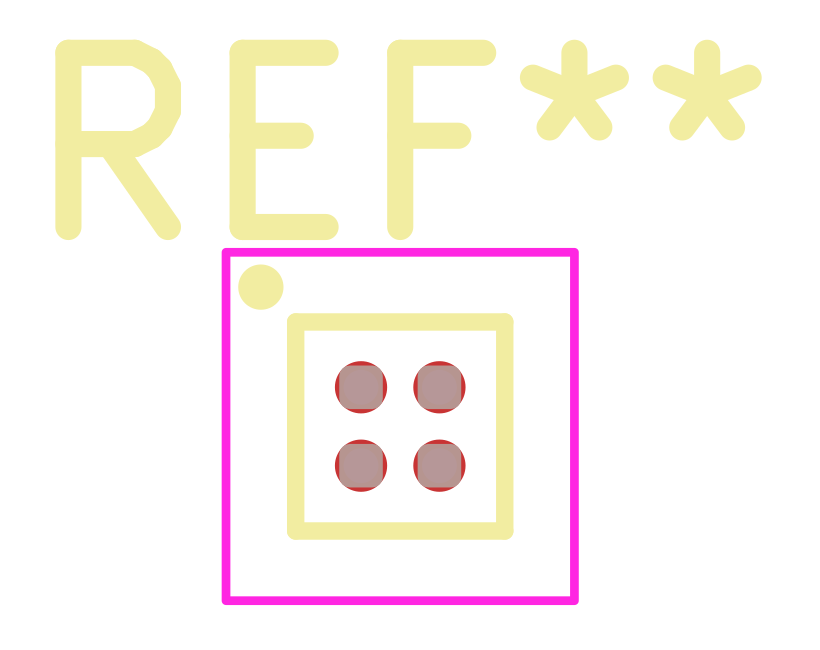
\includegraphics[width=\linewidth]{figures/EPC2036_LGA4_SMD_P0.45mm.png}\caption{EPC2036 (Q1)}\end{subfigure}\hfill
\begin{subfigure}[b]{0.32\textwidth}\centering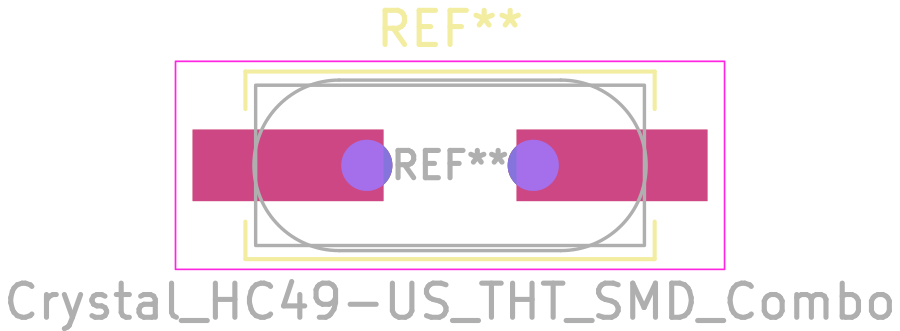
\includegraphics[width=\linewidth]{figures/Crystal_HC49-US_THT_SMD_Combo.png}\caption{HC-49 combo (Y1)}\end{subfigure}\hfill
\begin{subfigure}[b]{0.32\textwidth}\centering
\includegraphics[width=\linewidth]{figures/C_Trimmer_Voltronics_JZ.png}\caption{JZ trimmer (C9)}\end{subfigure}\\[0.6em]
\begin{subfigure}[b]{0.36\textwidth}\centering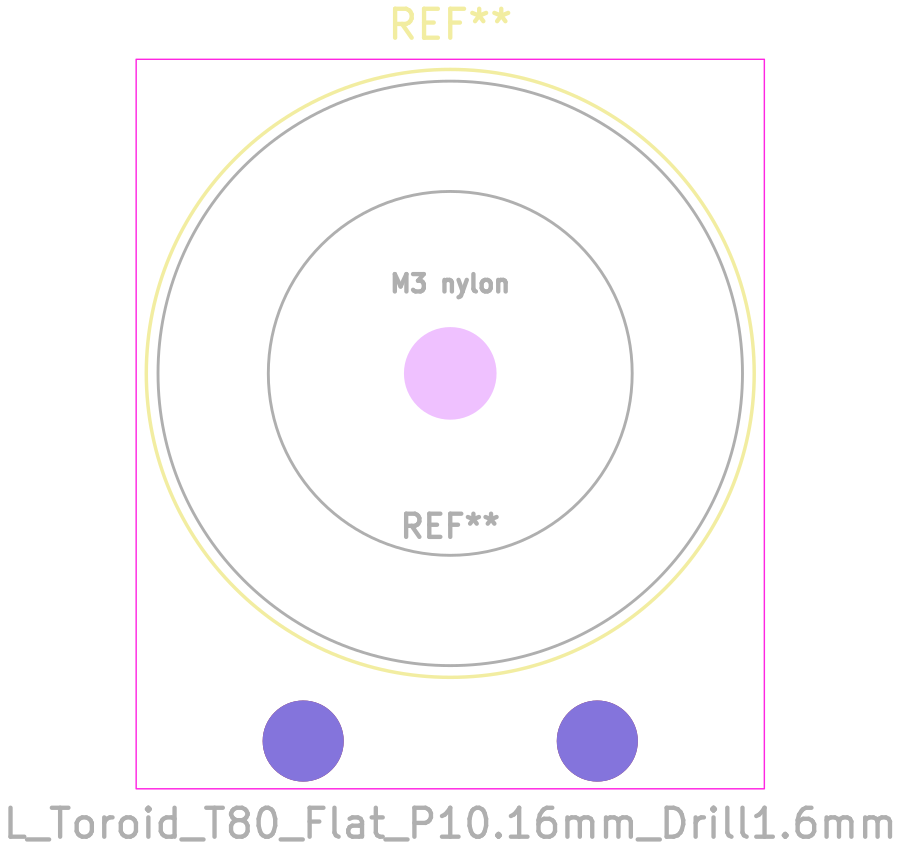
\includegraphics[width=\linewidth]{figures/L_Toroid_T80_Flat_P10.16mm_Drill1.6mm.png}\caption{T-80 flat (L2, L3)}\end{subfigure}\hspace{2em}
\begin{subfigure}[b]{0.36\textwidth}\centering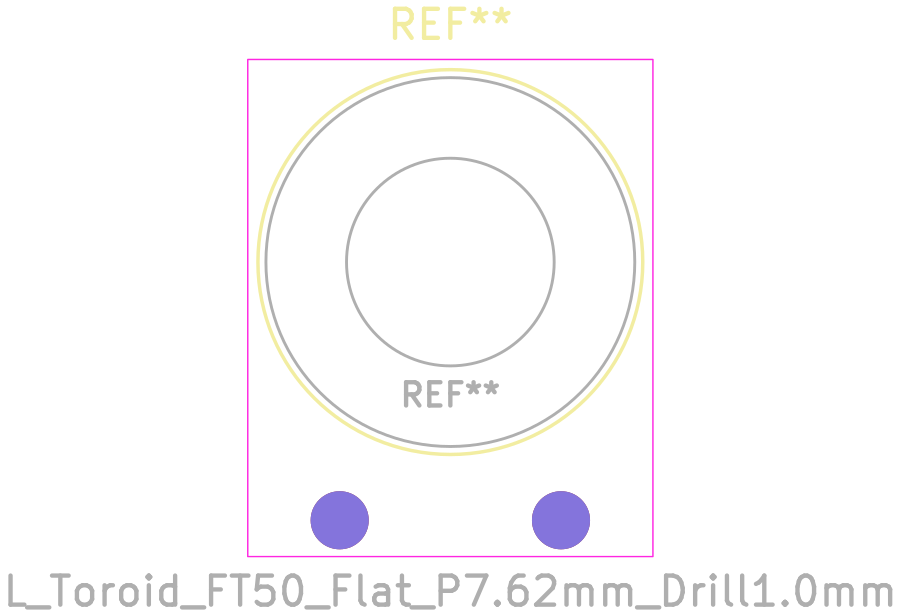
\includegraphics[width=\linewidth]{figures/L_Toroid_FT50_Flat_P7.62mm_Drill1.0mm.png}\caption{FT-50 flat (L1)}\end{subfigure}
\caption{Project footprints rendered with \texttt{kicad-cli} (not to the same scale). Yellow: silkscreen; magenta: courtyard; grey: fabrication outline.}\label{fig:fp}
\end{figure}

%=====================================================================
\section{Simulation results}\label{sec:sim}

\subsection{Setup and models}
All simulations are ngspice 44.2 transients of the schematic at \SI{12.0}{\volt} and \SI{7.030}{\mega\hertz}, 300 cycles from initial conditions (L1 at \SI{0.35}{\ampere}, C2 at \SI{12}{\volt}). The 100-cycle analysis window matches the preceding 100 cycles to within 0.01\,\%, and harmonics come from a coherent FFT over exactly 100 cycles, cross-checked with a Blackman window \cite{projsim,projnotes}. Q1 is EPC's own EPC2036 model from its GaN device library, translated from LTspice syntax for ngspice (\texttt{if()} to \texttt{?:}, \texttt{log()} to \texttt{ln()}, junction fixed at \SI{25}{\celsius}); its parameters match EPC's Spectre file line for line. The translated model gives $C_{oss}=\SI{50.4}{\pico\farad}$ at \SI{50}{\volt}, a charge-equivalent $C_{oss}$ of \SI{82}{\pico\farad} from 0 to \SI{42.7}{\volt}, and \SI{50}{\milli\ohm} at $V_{GS}=\SI{5}{\volt}$, \SI{1}{\ampere} (datasheet maximum \SI{73}{\milli\ohm}) \cite{projnotes,epc2036ds}. Losses: L1 \SI{37}{\milli\ohm} copper plus \SI{277}{\kilo\ohm} core $R_p$; L2 $Q_u=330$ (\SI{0.292}{\ohm}); L3 $Q_u=320$ (\SI{0.105}{\ohm}); C0G ESR \SI{20}{\milli\ohm} or $Q=1000$. Drive is an ideal 0--\SI{5}{\volt} square with \SI{1}{\nano\second} edges, \SI{7}{\ohm} source resistance and \SI{2}{\nano\henry} gate loop. These are estimates \cite{projnotes}. The oscillator uses a Fairchild 2N3904 model and a placeholder crystal; keying uses a level-1 AO3407A model fitted to the datasheet; U1 is a behavioural Schmitt trigger.

\subsection{Waveforms and spectrum}
Figure~\ref{fig:wave} shows drain and gate voltage. Without the filter (Table~\ref{tab:c1sweep}) the second harmonic at \SI{50}{\ohm} is about \SI{-27}{dBc}, better than Sokal's tank-only \SI{-20}{dBc} because the L-match shunt C3 adds about \SI{7}{\decibel} \cite{projnotes}. With the elliptic filter (Table~\ref{tab:simlpf}, Figure~\ref{fig:spec}) every harmonic is at least \SI{18.9}{\decibel} below the FCC limit and \SI{8.9}{\decibel} below the \SI{-53}{dBc} target; $3f$ is the closest. The \SI{-82}{dBc} at $2f$ assumes the trap is exactly on \SI{14.06}{\mega\hertz}; with the trap inductor off by $\pm$10\,\%, $2f$ was \SI{-54}{} to \SI{-63}{dBc} \cite{projsim}.

\begin{figure}[h]
\centering
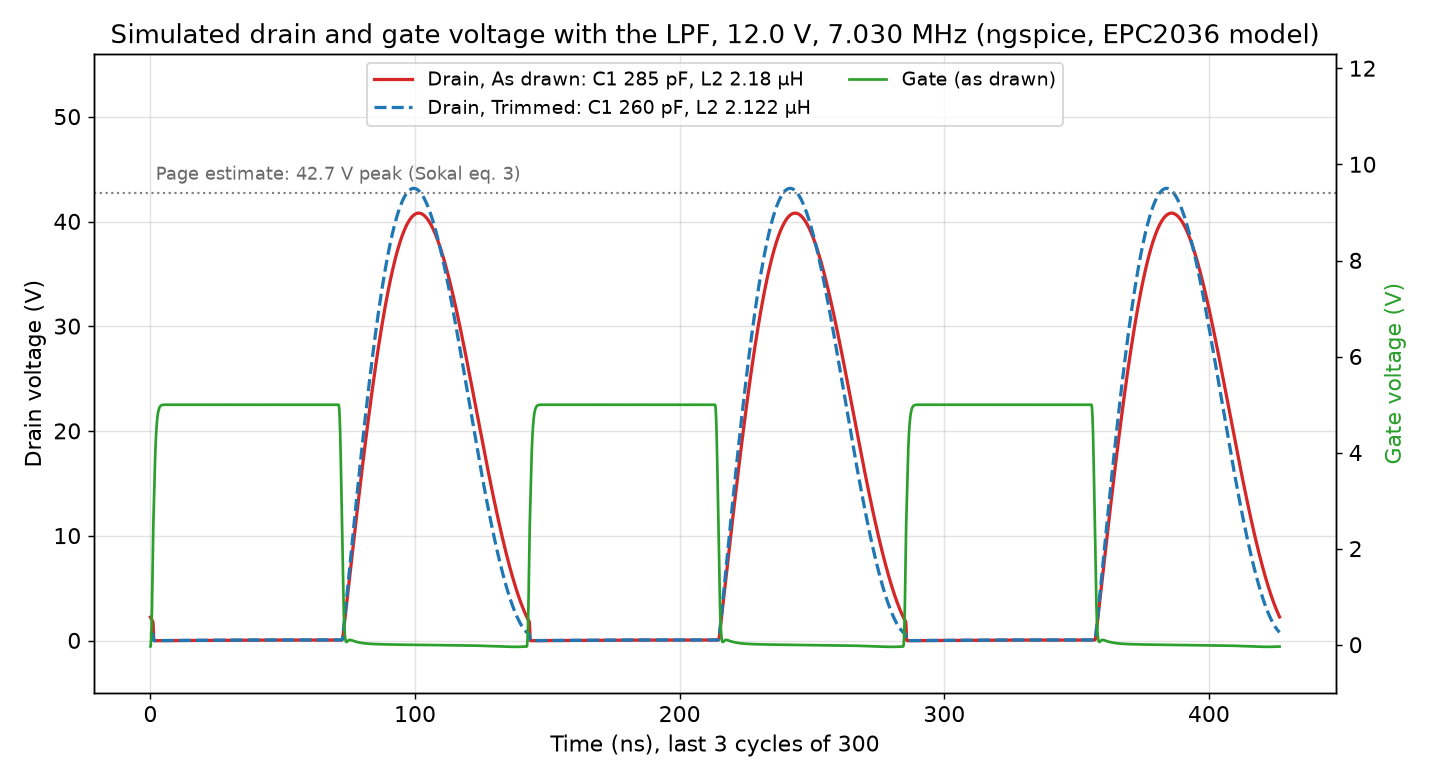
\includegraphics[width=0.92\textwidth]{figures/waveforms_lpf.png}
\caption{Simulated drain and gate voltage with the LPF, as drawn (C1 \SI{285}{\pico\farad}, L2 \SI{2.18}{\micro\henry}) and trimmed (C1 \SI{260}{\pico\farad}, L2 \SI{2.122}{\micro\henry}) \cite{projsim}.}\label{fig:wave}
\end{figure}

\begin{figure}[h]
\centering
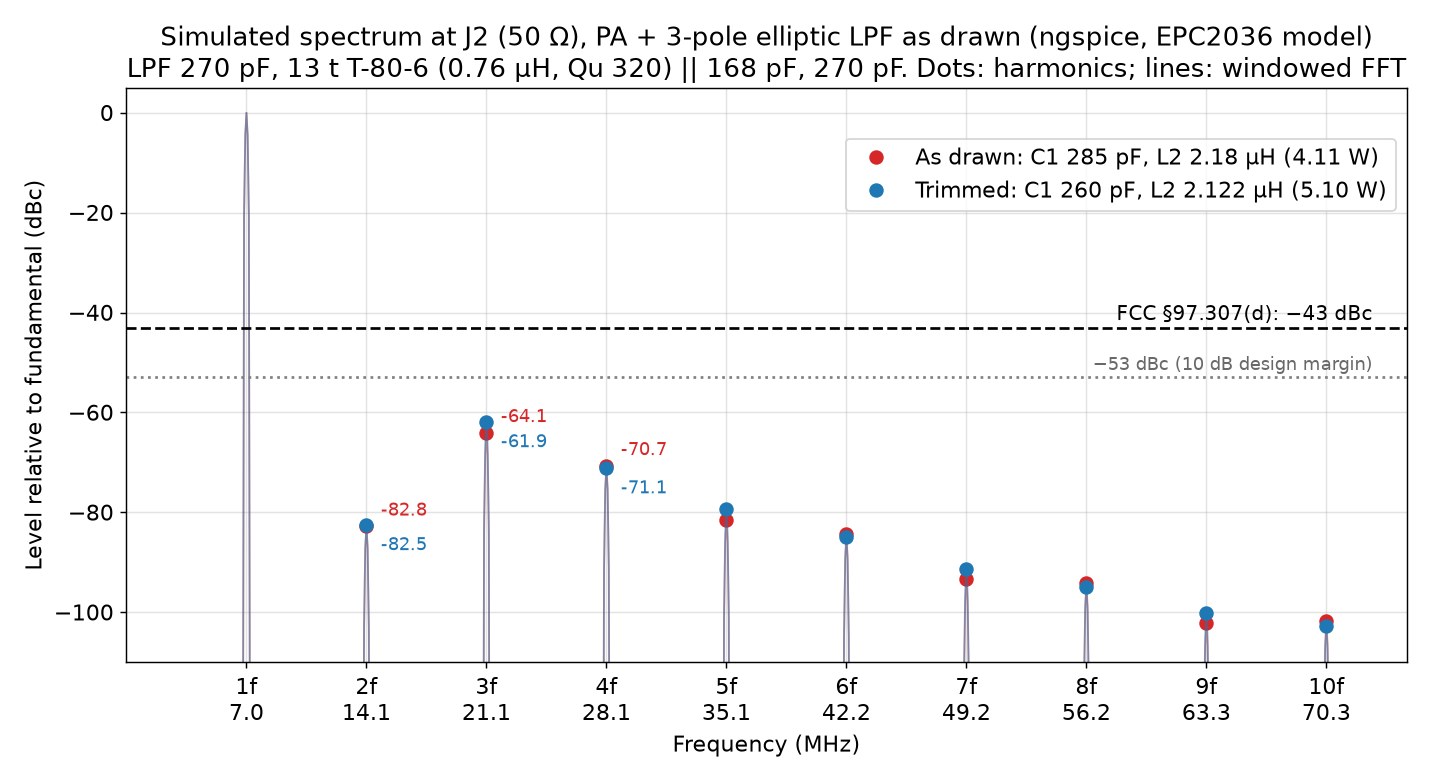
\includegraphics[width=0.92\textwidth]{figures/spectrum_lpf.png}
\caption{Simulated spectrum at J2 with the 3-pole elliptic LPF \cite{projsim}.}\label{fig:spec}
\end{figure}

\begin{figure}[h]
\centering
\begin{subfigure}[b]{0.49\textwidth}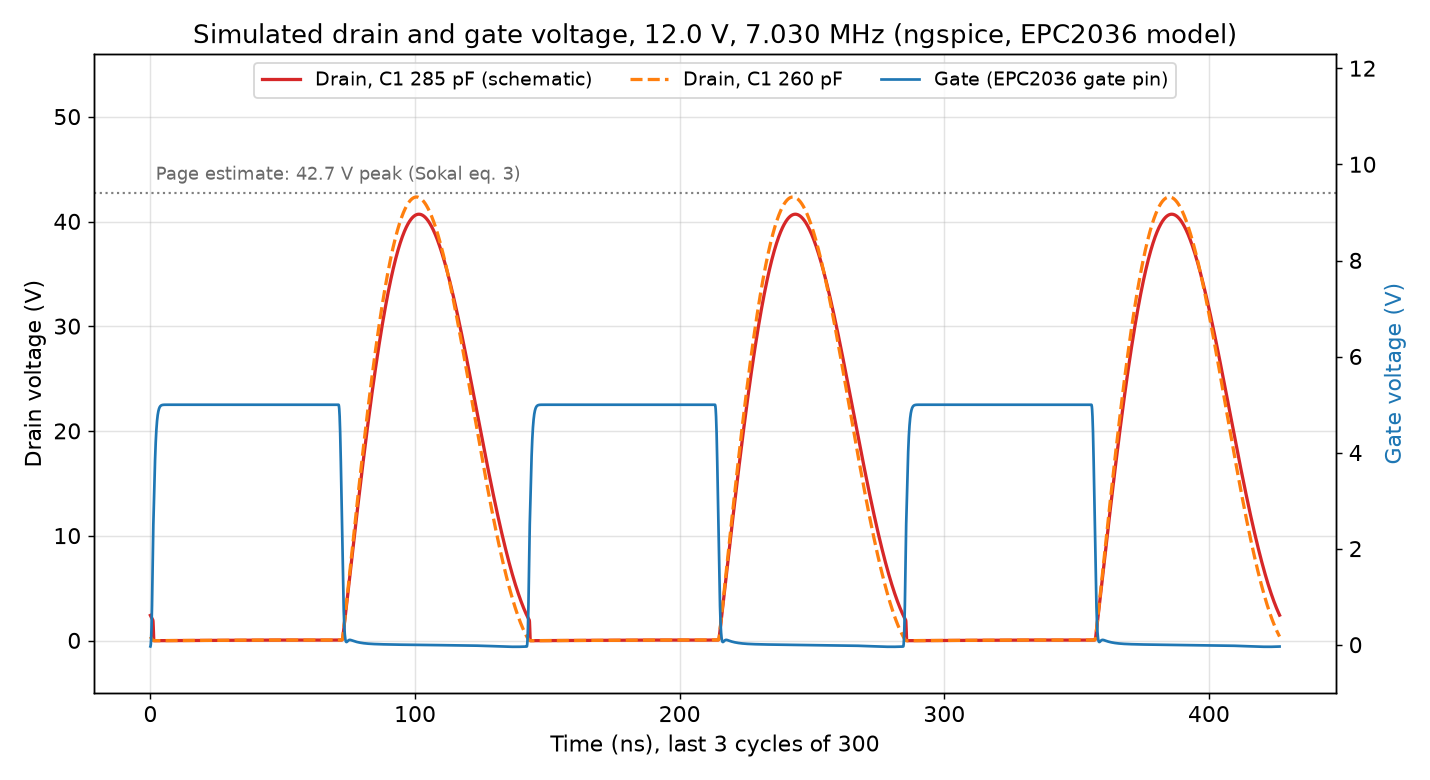
\includegraphics[width=\linewidth]{figures/waveforms_nolpf.png}\caption{Waveforms, no LPF}\end{subfigure}\hfill
\begin{subfigure}[b]{0.49\textwidth}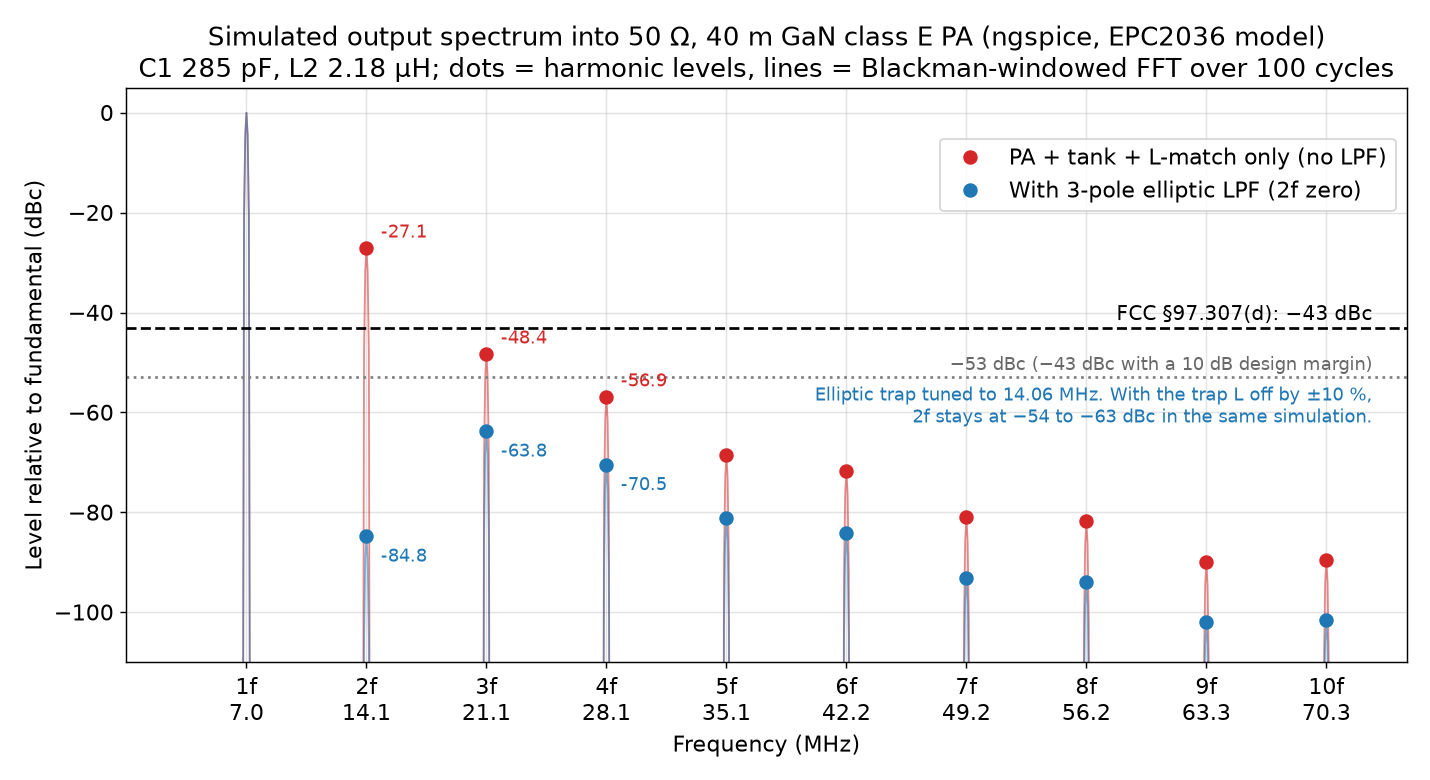
\includegraphics[width=\linewidth]{figures/spectrum_nolpf.png}\caption{Spectrum, no LPF}\end{subfigure}
\caption{PA alone into \SI{50}{\ohm} (C1 \SI{285}{\pico\farad}, L2 \SI{2.18}{\micro\henry}) \cite{projsim}.}\label{fig:nolpf}
\end{figure}

\begin{table}[h]
\centering\small
\caption{PA with the elliptic LPF as drawn (L3 13\,t T-80-6, \SI{0.7605}{\micro\henry}, $Q_u$ 320; C17+C18 \SI{168}{\pico\farad}) \cite{projsim} (\texttt{v2/results\_v2.json}). Values exclude gate drive.}\label{tab:simlpf}
\begin{tabular}{@{}lrr@{}}
\toprule
Quantity & As drawn (C1 285, L2 2.18) & Trimmed (C1 260, L2 2.122) \\ \midrule
Output at J2 (fundamental) & \SI{4.11}{\watt} & \SI{5.10}{\watt} \\
DC in (PA rail) & \SI{4.27}{\watt} (\SI{356}{\milli\ampere}) & \SI{5.29}{\watt} (\SI{441}{\milli\ampere}) \\
Drain efficiency & \SI{96.4}{\percent} & \SI{96.4}{\percent} \\
Peak drain voltage & \SI{40.8}{\volt} & \SI{43.2}{\volt} \\
Drain voltage at turn-on & \SI{1.9}{\volt} & \SI{0.65}{\volt} \\
LPF loss & \SI{27}{\milli\watt} (0.66\,\%) & \SI{34}{\milli\watt} (0.66\,\%) \\
$2f$ / $3f$ / $4f$ / $5f$ & $-82.8$ / $-64.1$ / $-70.7$ / $-81.5$\,dBc & $-82.5$ / $-61.9$ / $-71.1$ / $-79.4$\,dBc \\
$6f$--$10f$ & $\leq\SI{-84.4}{dBc}$ & $\leq\SI{-85.0}{dBc}$ \\
Gate voltage range & \SIrange{-0.04}{5.00}{\volt} & \SIrange{-0.04}{5.00}{\volt} \\
\bottomrule
\end{tabular}
\end{table}

\subsection{Output versus supply}
Table~\ref{tab:vsweep} and Figure~\ref{fig:vsweep} show the trimmed PA plus LPF at reduced rail voltages. Output scales with the square of the rail within 5\,\% and the DC input resistance stays near \SI{28}{\ohm}, which makes the low-voltage points useful for bring-up \cite{projsim}. With the rail at \SI{0}{\volt} and drive running, \SI{8.0}{\micro\watt} (\SI{-58.1}{dBc}) leaks through Q1's capacitances.

\begin{table}[h]
\centering\small
\begin{minipage}[c]{0.5\textwidth}\centering
\captionof{table}{Supply sweep, trimmed + LPF \cite{projsim} (\texttt{v3/results\_v3.json}).}\label{tab:vsweep}
\begin{tabular}{@{}rrrr@{}}
\toprule
Rail & Output at J2 & Rail current & DC res. \\ \midrule
\SI{3}{\volt} & \SI{0.304}{\watt} & \SI{105}{\milli\ampere} & \SI{28.5}{\ohm} \\
\SI{6}{\volt} & \SI{1.238}{\watt} & \SI{214}{\milli\ampere} & \SI{28.0}{\ohm} \\
\SI{9}{\volt} & \SI{2.831}{\watt} & \SI{327}{\milli\ampere} & \SI{27.6}{\ohm} \\
\SI{12}{\volt} & \SI{5.101}{\watt} & \SI{441}{\milli\ampere} & \SI{27.2}{\ohm} \\
\bottomrule
\end{tabular}
\end{minipage}\hfill
\begin{minipage}[c]{0.46\textwidth}\centering
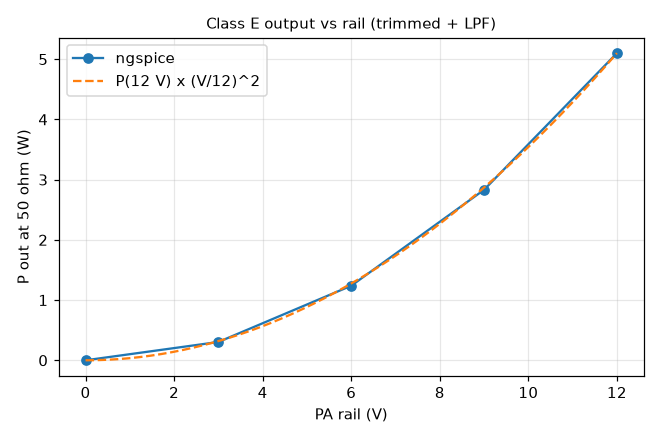
\includegraphics[width=\linewidth]{figures/pout_vs_vdd_v3.png}
\captionof{figure}{Output versus PA rail \cite{projsim}.}\label{fig:vsweep}
\end{minipage}
\end{table}

\subsection{Keying and oscillator}
Figure~\ref{fig:keying} shows the keyed rail and RF envelope for C4 values (timing in Table~\ref{tab:keying}); the envelope has straight sides from the near-linear rail ramp and rounded corners from the gate RC. Spectral clicks from this shape were not simulated \cite{projsim,projnotes}. Figure~\ref{fig:osc} shows the oscillator: clean switching at U1 from \SI{0.65}{\milli\second} after power-up and settled by about \SI{2}{\milli\second}, a collector swing of \SI{3.28}{\volt}~p-p, \SI{1.98}{\milli\ampere} rms crystal current and a 52.9\,\% duty cycle at U1's output \cite{projsim}. Start-up time and frequency depend on the real crystal.

\begin{figure}[h]
\centering
\begin{subfigure}[b]{0.49\textwidth}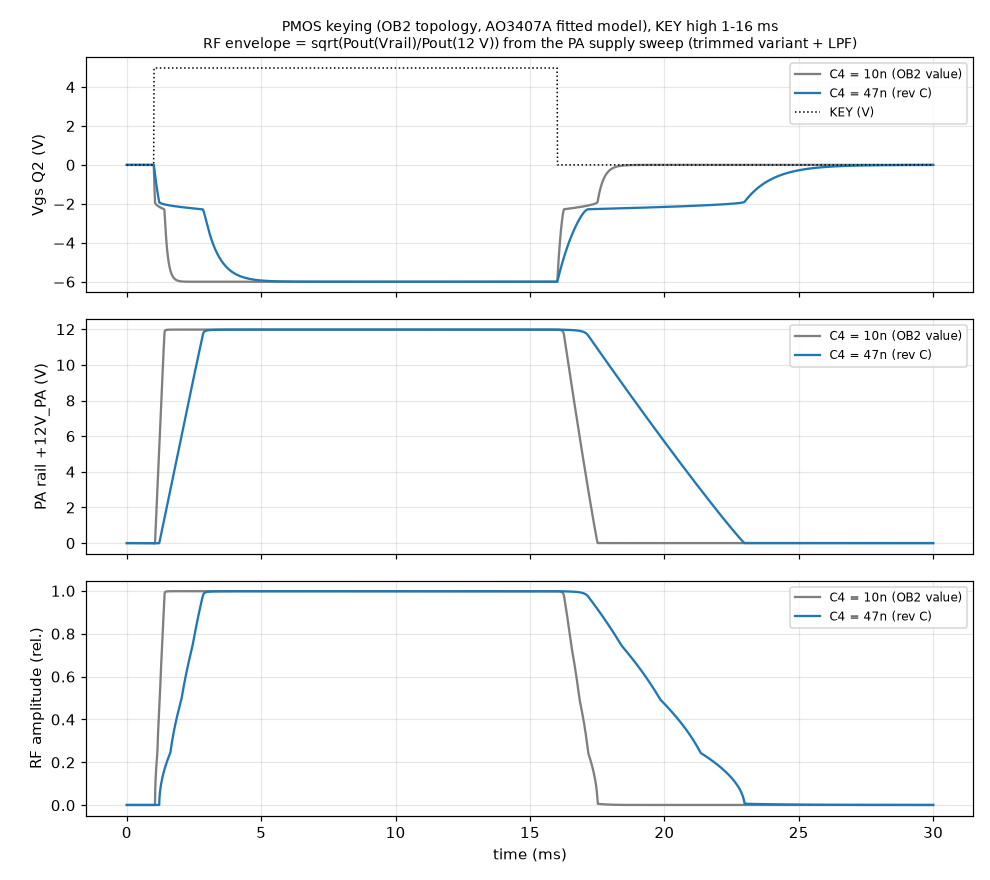
\includegraphics[width=\linewidth]{figures/keying_v3.png}\caption{Keying (rev 3 topology; rev 4 timing identical)}\label{fig:keying}\end{subfigure}\hfill
\begin{subfigure}[b]{0.49\textwidth}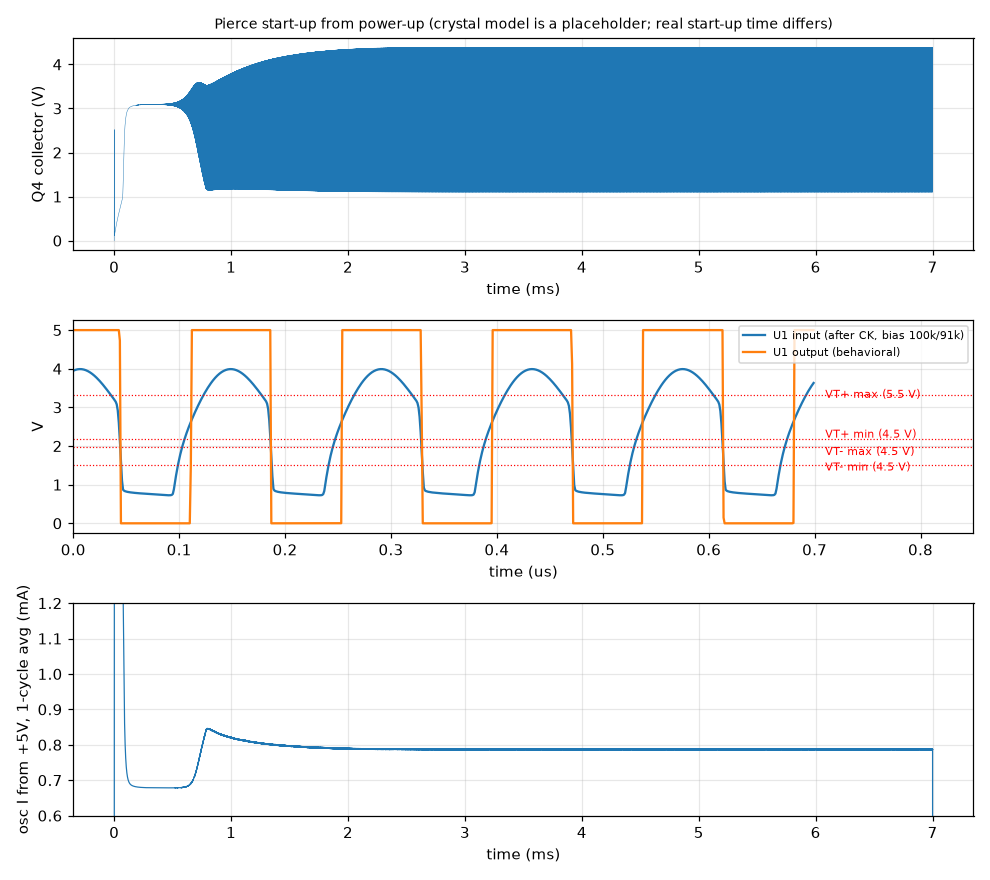
\includegraphics[width=\linewidth]{figures/osc_v3.png}\caption{Pierce oscillator start-up and U1 input}\label{fig:osc}\end{subfigure}
\caption{Simulated keying envelope and oscillator \cite{projsim}.}
\end{figure}

\subsection{Gate R1 and clamp study (rev 6)}\label{sec:gatesim}
The trimmed PA + LPF deck (C1 \SI{260}{\pico\farad}, L2 \SI{2.122}{\micro\henry}, EPC's EPC2036 model) was re-run with R1 = 0, 1, 2.2, 3.3, 4.7 and \SI{10}{\ohm}. The gate-loop inductance was set to 0, 1 and \SI{2}{\nano\henry} (\SI{2}{\nano\henry} is the earlier baseline), plus a \SI{5}{\nano\henry} stress case. Then Diodes Inc.\ manufacturer models of a BAT54 Schottky and BZX84C5V6 and BZX84C6V2 zeners were added from gate pad to source, alone and in pairs \cite{diodesSpice}. Diodes Inc.\ publishes no single-SOT-23 BAT54 model, so the BAT54W (SOT-323) model stands in for it. The driver is modelled as before.

\emph{Assumed parasitics:} the \SI{7}{\ohm} driver resistance and 1\,ns edges; the loop inductance lumped between R1 and the gate pad; no common-source inductance; no clamp lead inductance; no probe loading. The model's internal gate resistance is \SI{0.6}{\ohm}. Gate voltages are at the pad; the internal gate node differed by no more than about \SI{0.02}{\volt}. The gate-drive current is the mean current from the \SI{5}{\volt} source, and the whole-transmitter efficiency uses the Table~\ref{tab:budget} overheads \cite{projsim}. TI's TPD1E and Nexperia's PESD5V0 TVS parts were not simulated because no vendor model was obtained (the Nexperia site refused the download).

\begin{table}[p]\centering\footnotesize\setlength{\tabcolsep}{3.5pt}
\caption{Gate R1 and gate-loop inductance sweep, trimmed PA + LPF at \SI{12.0}{\volt}\simv. Driver as before: ideal 0--5\,V, 1\,ns edges, \SI{7}{\ohm} output (estimate). Loop L is assumed and lumped between R1 and the Q1 gate pad; 5\,nH is a stress case. Whole-transmitter efficiency uses the Table~\ref{tab:budget} overheads with the simulated gate-drive power; $\Delta$ is in percentage points against R1 \SI{0}{\ohm}, 2\,nH (the earlier baseline) \cite{projsim}.}\label{tab:gate-r1}
\begin{tabular}{@{}llrrrrrrr@{}}\toprule
Loop L & R1 ($\Omega$) & $P_{out}$ (W) & $\eta_D$ (\%) & $\eta_{tot}$ (\%) & $\Delta\eta_{tot}$ (pts) & $V_{g,max}$ (V) & $V_{g,min}$ (V) & $I_{5V,gate}$ (mA) \\ \midrule
\multirow{6}{*}{0\,nH}  & 0 & 5.101 & 96.37 & 95.66 & +0.041 & 5.00 & $-$0.04 & 2.87 \\
 & 1 & 5.101 & 96.37 & 95.64 & +0.028 & 5.00 & $-$0.05 & 2.98 \\
 & 2.2 & 5.101 & 96.36 & 95.63 & +0.014 & 5.00 & $-$0.06 & 3.08 \\
 & 3.3 & 5.101 & 96.36 & 95.62 & +0.002 & 5.00 & $-$0.06 & 3.16 \\
 & 4.7 & 5.102 & 96.35 & 95.60 & $-$0.011 & 5.00 & $-$0.07 & 3.25 \\
 & 10 & 5.103 & 96.33 & 95.56 & $-$0.055 & 5.00 & $-$0.10 & 3.49 \\
\midrule
\multirow{6}{*}{1\,nH}  & 0 & 5.101 & 96.37 & 95.63 & +0.018 & 5.00 & $-$0.04 & 3.12 \\
 & 1 & 5.101 & 96.37 & 95.62 & +0.008 & 5.00 & $-$0.05 & 3.18 \\
 & 2.2 & 5.101 & 96.36 & 95.61 & $-$0.002 & 5.00 & $-$0.06 & 3.26 \\
 & 3.3 & 5.101 & 96.36 & 95.60 & $-$0.011 & 5.00 & $-$0.06 & 3.31 \\
 & 4.7 & 5.102 & 96.36 & 95.59 & $-$0.022 & 5.00 & $-$0.07 & 3.38 \\
 & 10 & 5.103 & 96.34 & 95.56 & $-$0.060 & 5.00 & $-$0.10 & 3.56 \\
\midrule
\multirow{6}{*}{2\,nH}  & 0 & 5.101 & 96.37 & 95.62 & +0.000 & 5.00 & $-$0.04 & 3.31 \\
 & 1 & 5.101 & 96.37 & 95.61 & $-$0.007 & 5.00 & $-$0.05 & 3.35 \\
 & 2.2 & 5.101 & 96.37 & 95.60 & $-$0.015 & 5.00 & $-$0.06 & 3.40 \\
 & 3.3 & 5.101 & 96.36 & 95.59 & $-$0.022 & 5.00 & $-$0.06 & 3.44 \\
 & 4.7 & 5.102 & 96.36 & 95.59 & $-$0.031 & 5.00 & $-$0.07 & 3.48 \\
 & 10 & 5.103 & 96.34 & 95.55 & $-$0.065 & 5.00 & $-$0.10 & 3.62 \\
\midrule
\multirow{6}{*}{5\,nH (stress)}  & 0 & 5.101 & 96.37 & 95.59 & $-$0.028 & 5.38 & $-$0.64 & 3.61 \\
 & 1 & 5.101 & 96.37 & 95.58 & $-$0.032 & 5.21 & $-$0.38 & 3.62 \\
 & 2.2 & 5.101 & 96.37 & 95.58 & $-$0.036 & 5.08 & $-$0.13 & 3.64 \\
 & 3.3 & 5.101 & 96.37 & 95.58 & $-$0.041 & 5.01 & $-$0.06 & 3.66 \\
 & 4.7 & 5.102 & 96.36 & 95.57 & $-$0.046 & 5.00 & $-$0.07 & 3.68 \\
 & 10 & 5.103 & 96.34 & 95.54 & $-$0.072 & 5.00 & $-$0.10 & 3.75 \\
\bottomrule
\end{tabular}\end{table}

\begin{table}[tbp]\centering\footnotesize\setlength{\tabcolsep}{3.5pt}
\caption{Gate-source clamps at the Q1 gate pad (Diodes Inc. models \cite{diodesSpice}), trimmed PA + LPF\simv. Columns as Table~\ref{tab:gate-r1}; $P_{cl}$ is the power dissipated in the clamp model \cite{projsim}.}\label{tab:gate-clamp}
\begin{tabular}{@{}lllrrrrrr@{}}\toprule
Loop L & R1 ($\Omega$) & Clamp & $\eta_{tot}$ (\%) & $\Delta\eta_{tot}$ (pts) & $V_{g,max}$ (V) & $V_{g,min}$ (V) & $I_{5V,gate}$ (mA) & $P_{cl}$ (mW) \\ \midrule
2\,nH & 0 & none & 95.62 & +0.000 & 5.00 & $-$0.04 & 3.31 & 0.00 \\
 &  & BAT54W & 95.58 & $-$0.035 & 5.00 & $-$0.04 & 3.64 & 0.10 \\
 &  & BZX84C5V6 & 95.48 & $-$0.141 & 5.00 & $-$0.04 & 4.64 & 3.58 \\
 &  & BZX84C6V2 & 95.50 & $-$0.120 & 5.00 & $-$0.04 & 4.44 & 2.86 \\
 &  & BAT54W + C5V6 & 95.44 & $-$0.176 & 5.00 & $-$0.04 & 4.97 & 3.61 \\
 &  & BAT54W + C6V2 & 95.46 & $-$0.156 & 5.00 & $-$0.04 & 4.78 & 2.89 \\
\midrule
2\,nH & 2.2 & none & 95.60 & $-$0.015 & 5.00 & $-$0.06 & 3.40 & 0.00 \\
 &  & BAT54W & 95.57 & $-$0.051 & 5.00 & $-$0.06 & 3.73 & 0.10 \\
 &  & BZX84C5V6 & 95.46 & $-$0.159 & 5.00 & $-$0.05 & 4.74 & 3.09 \\
 &  & BZX84C6V2 & 95.48 & $-$0.138 & 5.00 & $-$0.05 & 4.54 & 2.44 \\
 &  & BAT54W + C5V6 & 95.42 & $-$0.195 & 5.00 & $-$0.05 & 5.07 & 3.10 \\
 &  & BAT54W + C6V2 & 95.44 & $-$0.174 & 5.00 & $-$0.05 & 4.88 & 2.47 \\
\midrule
5\,nH & 0 & none & 95.59 & $-$0.028 & 5.38 & $-$0.64 & 3.61 & 0.00 \\
 &  & BAT54W & 95.55 & $-$0.064 & 5.35 & $-$0.28 & 3.95 & 0.10 \\
 &  & BZX84C5V6 & 95.45 & $-$0.169 & 5.05 & $-$0.14 & 4.94 & 3.93 \\
 &  & BZX84C6V2 & 95.47 & $-$0.149 & 5.11 & $-$0.19 & 4.75 & 3.16 \\
 &  & BAT54W + C5V6 & 95.41 & $-$0.205 & 5.05 & $-$0.08 & 5.28 & 3.94 \\
 &  & BAT54W + C6V2 & 95.43 & $-$0.184 & 5.10 & $-$0.12 & 5.09 & 3.17 \\
\bottomrule
\end{tabular}\end{table}
\begin{table}[tbp]\centering\small
\caption{Clamp DC behaviour: model (ngspice DC sweep of the Diodes Inc. models \cite{diodesSpice}) against the onsemi datasheet limits \cite{onsemiBZX84,onsemiBAT54}. The EPC2036 gate is rated \SI{6}{\volt} / \SI{-4}{\volt}, with up to \SI{0.9}{\milli\ampere} forward gate leakage at \SI{5}{\volt} \cite{epc2036ds}.}\label{tab:clamp-dc}
\begin{tabularx}{\textwidth}{@{}L{3.6cm}L{2.7cm}L{2.7cm}Y@{}}\toprule
Quantity & BZX84C5V6 & BZX84C6V2 & BAT54 \\ \midrule
Leakage at \SI{5.0}{\volt}, model & \SI{11.4}{\micro\ampere} & \SI{0.03}{\nano\ampere} & \SI{34.9}{\micro\ampere} (equal to the model's IS; an artefact) \\
Leakage, datasheet max & \SI{1}{\micro\ampere} at \SI{2}{\volt} & \SI{3}{\micro\ampere} at \SI{4}{\volt} & \SI{2}{\micro\ampere} at \SI{25}{\volt} \\
Clamp voltage at 1 / 5 / 20\,mA, model & 5.37 / 5.59 / 6.07\,V & 6.13 / 6.20 / 6.29\,V & -- \\
$V_Z$ datasheet (min--max) at 1 / 5 / 20\,mA & 4.8--6.0 / 5.2--6.0 / 5.2--6.3\,V & 5.6--6.6 / 5.8--6.6 / 5.8--6.8\,V & -- \\
Forward voltage at \SI{10}{\milli\ampere}, model & 0.90\,V & 0.90\,V & 0.34\,V (datasheet 0.35 typ, 0.40 max) \\
Capacitance & model CJO \SI{57.6}{\pico\farad}; datasheet \SI{200}{\pico\farad} at \SI{0}{\volt} & model CJO \SI{49.4}{\pico\farad}; datasheet \SI{185}{\pico\farad} at \SI{0}{\volt} & model CJO \SI{13.3}{\pico\farad}; datasheet 7.6 typ, \SI{10}{\pico\farad} max at \SI{1}{\volt} \\
\bottomrule\end{tabularx}\end{table}


\begin{figure}[tbp]
\centering
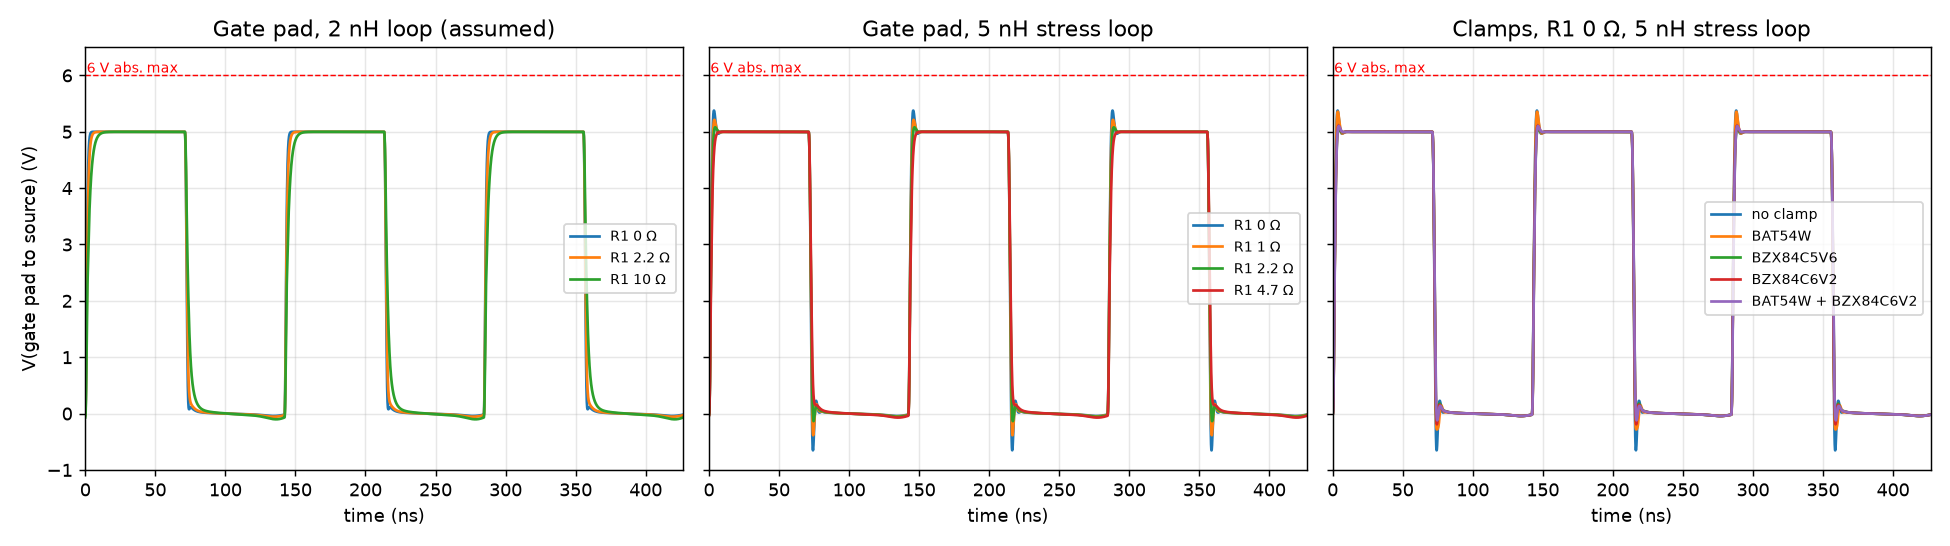
\includegraphics[width=\textwidth]{figures/gate_v5.png}
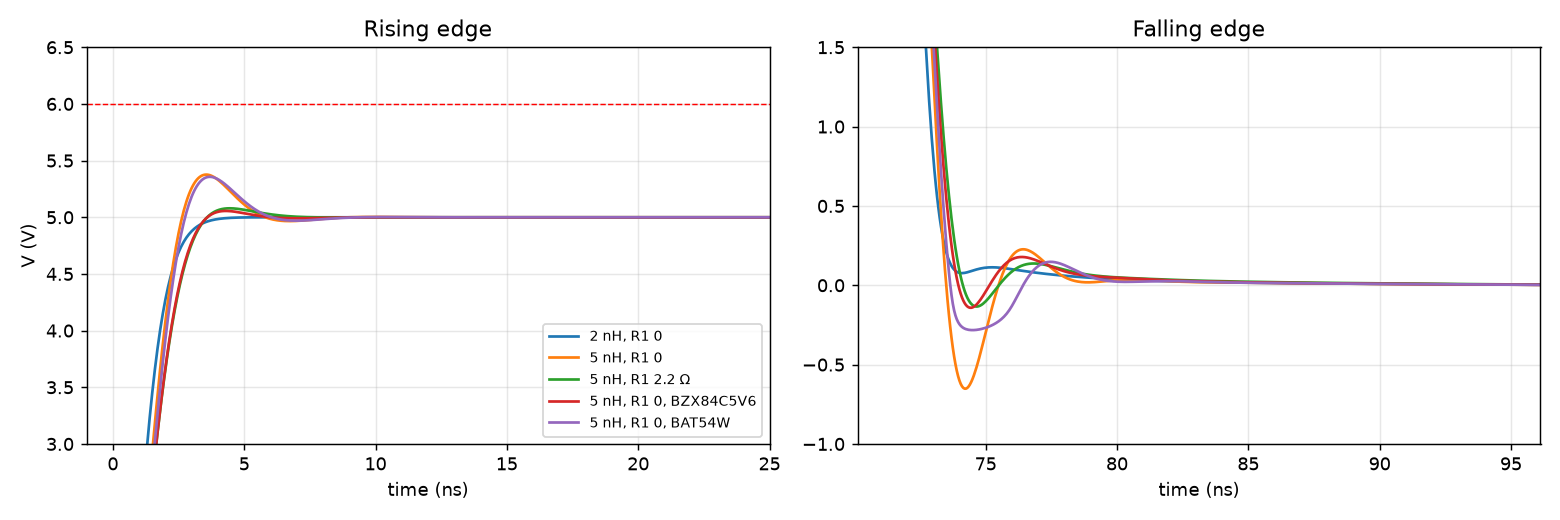
\includegraphics[width=0.9\textwidth]{figures/gate_edges_v5.png}
\caption{Simulated gate-pad voltage over three RF cycles (top) and at the edges (bottom) for the key cases \cite{projsim}.}\label{fig:gatesim}
\end{figure}

\paragraph{Findings.}
\begin{itemize}[nosep]
\item Up to \SI{2}{\nano\henry}, the gate never exceeds \SI{5.00}{\volt} or goes below \SI{-0.10}{\volt}, for any R1. Output power is unchanged at \SI{5.10}{\watt}. R1 costs 0.007 (\SI{1}{\ohm}), 0.015 (\SI{2.2}{\ohm}) and 0.065 points (\SI{10}{\ohm}) of whole-transmitter efficiency at \SI{2}{\nano\henry}. The losses come from a slower turn-on, which raises the drain voltage at turn-on from 0.65 to \SI{0.85}{\volt} at \SI{10}{\ohm}, and from the 5\,V gate current rising from 3.31 to \SI{3.62}{\milli\ampere}.
\item Loop inductance is cheap to remove: \SI{0}{\nano\henry} is 0.04 points better than \SI{2}{\nano\henry} at R1 \SI{0}{\ohm}, because the 5\,V gate current drops from 3.31 to \SI{2.87}{\milli\ampere}.
\item At \SI{5}{\nano\henry} the gate overshoots to \SI{5.38}{\volt} and undershoots to \SI{-0.64}{\volt}, still inside the ratings. \SI{2.2}{\ohm} cuts this to \SI{5.08}{\volt} / \SI{-0.13}{\volt} for 0.008 points.
\item Clamps: the BAT54 alone costs 0.035 points (part of that is the model's \SI{35}{\micro\ampere} leakage, which is an artefact) and only limits undershoot. The zeners cost 0.12--0.14 points and the pairs 0.16--0.18 points, from the model's junction capacitance and series resistance. The datasheets give 185--\SI{200}{\pico\farad} at \SI{0}{\volt} against the models' 49--\SI{58}{\pico\farad}. An upper bound of $C V^2 f$ = \SI{185}{\pico\farad} $\times$ \SI{25}{\volt\squared} $\times$ \SI{7.03}{\mega\hertz} = \SI{33}{\milli\watt} at the 5\,V rail is about 0.67 points from \SI{12}{\volt}\est.
\item None of the clamps is tested in normal operation, because the unclamped gate stays under \SI{5.4}{\volt}. For a real transient the BZX84C6V2 sits above \SI{6}{\volt} at every current (model \SI{6.13}{\volt} at \SI{1}{\milli\ampere}, datasheet maximum \SI{6.8}{\volt} at \SI{20}{\milli\ampere}). The BZX84C5V6 holds about \SI{6.07}{\volt} at \SI{20}{\milli\ampere} in the model (datasheet maximum \SI{6.3}{\volt}) but leaks \SI{11}{\micro\ampere} at \SI{5}{\volt} in the model and may conduct at \SI{1}{\milli\ampere} from \SI{4.8}{\volt}. Neither clamp holds the gate under \SI{6}{\volt} with margin.
\end{itemize}
\textbf{Recommendation:} keep R1 at \SI{0}{\ohm} and the gate loop as short as possible, and leave D1 unfitted. Measure the gate at TP4/TP5 with a spring ground. Fit \SI{2.2}{\ohm} only if the gate exceeds about \SI{5.5}{\volt}. If the undershoot approaches \SI{-1}{\volt}, a BAT54 in D1 is the cheapest fix. A zener is not recommended.

\FloatBarrier
\subsection{Schematic as simulated}
Figure~\ref{fig:sch} is the rev 7 schematic (KiCad 9.0.2, ERC 0 violations). Revs 6 and 7 add only test points TP4--TP15, the DNP footprint D1 and the J1/J4 connector change to the rev 5 circuit. The connections are otherwise identical to rev 5, so the rev 5 simulations stand. A full-page copy is in Appendix~\ref{app:sch}.

\begin{figure}[h]
\centering
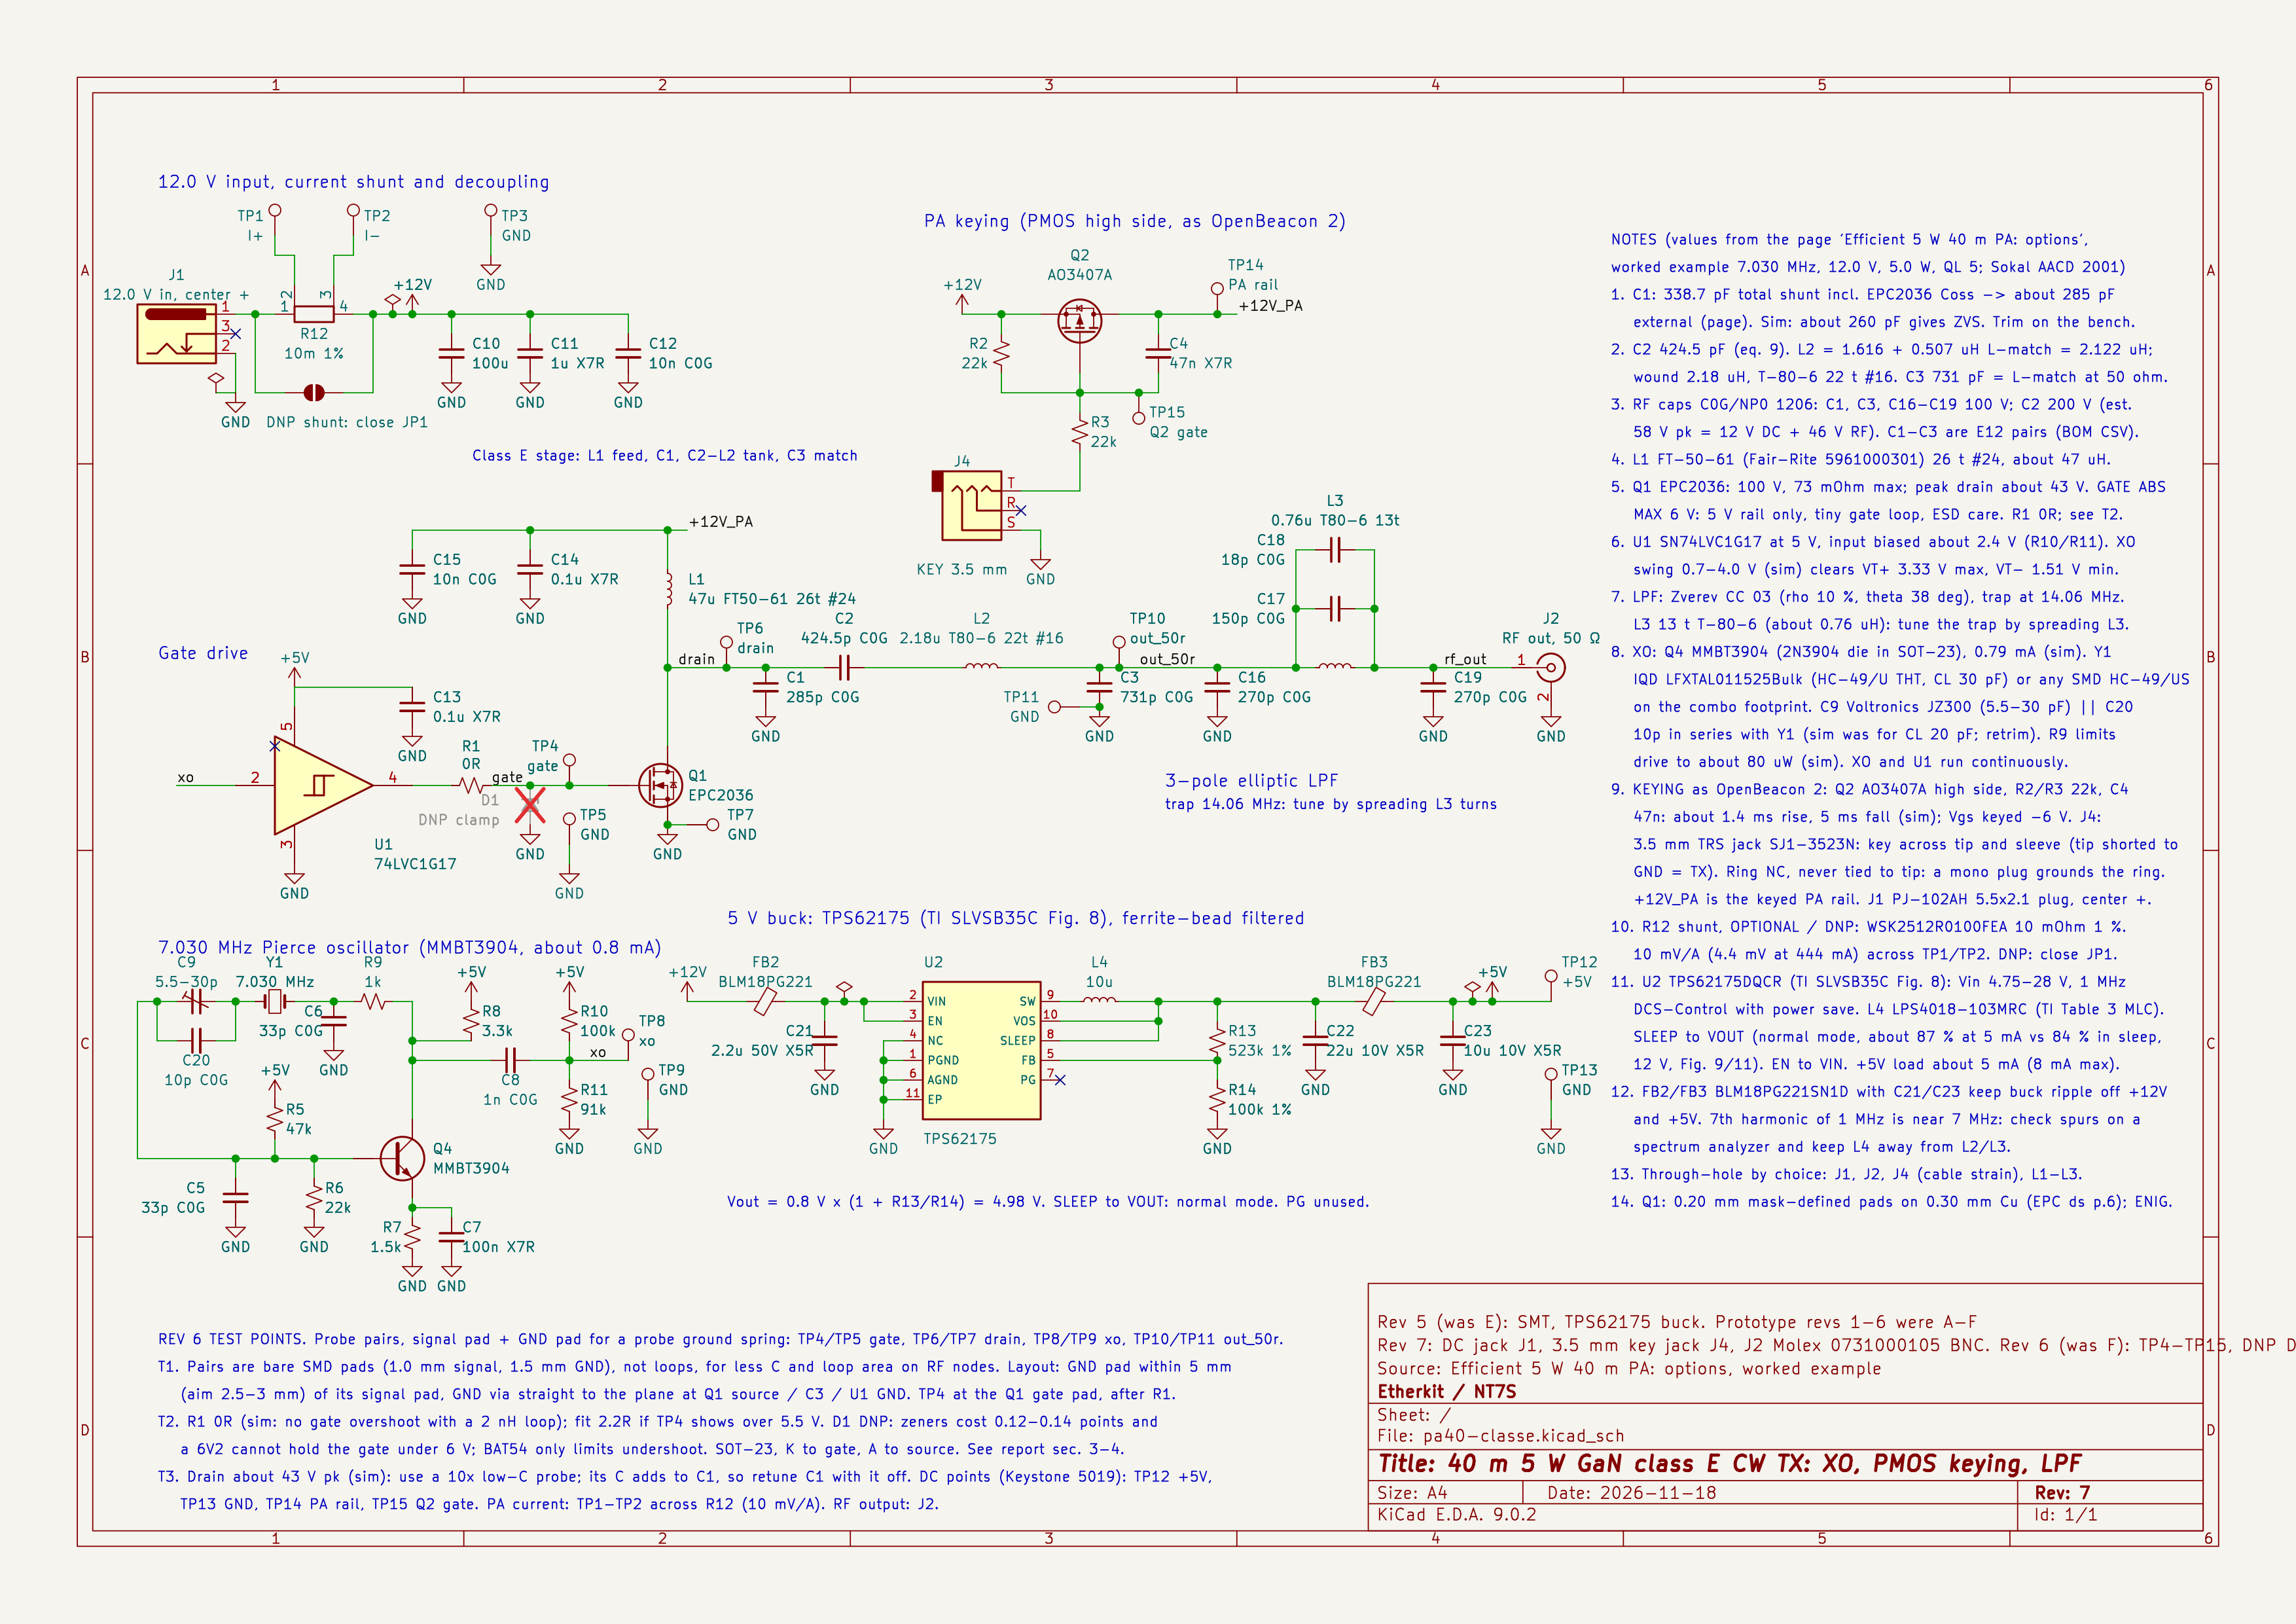
\includegraphics[width=\textwidth]{figures/schematic_rev7.png}
\caption{Rev 7 schematic \cite{projkicad}.}\label{fig:sch}
\end{figure}

%=====================================================================
\section{Power budget}\label{sec:budget}

Table~\ref{tab:budget} is the key-down budget at \SI{12.0}{\volt}, combining the trimmed PA + LPF run with the keying and oscillator runs and the TPS62175 efficiency of about \SI{87}{\percent} read from its datasheet curve \cite{projsim,tiTPS62175}. It is computed from the simulation JSON files by \texttt{report/gen\_tables.py} and \texttt{report/gen\_budget\_table.py}.

\begin{table}[h]\centering\small
\caption{Key-down power budget at \SI{12.0}{\volt} (simulated and estimated) \cite{projsim,projnotes,tiTPS62175}.}\label{tab:budget}
\begin{tabularx}{\textwidth}{@{}Yrl L{5.6cm}@{}}
\toprule Item & Power & Unit & Basis \\ \midrule
RF output at J2 & 5.101 & W & Trimmed PA + LPF run \\
PA rail input (drain, L1, tank, LPF) & 5.293 & W & Same run \\
\quad of which: LPF loss & 34.0 & mW & Power into C16 node minus power at J2 \\
\quad of which: Q1, L1, tank and L-match loss & 158.0 & mW & PA rail input minus LPF input \\
Q2 keying switch & 7.8 & mW & Keying run, fitted model \\
R2 + R3 divider while keyed & 3.3 & mW & $12^2/\SI{44}{\kilo\ohm}$ \\
5\,V loads from 12\,V via buck & 28.8 & mW & 25.1 mW / 0.87 (buck loss 3.7 mW) \\
\quad 5\,V load: Q1 gate drive & 16.6 & mW & Trimmed run, ideal driver \\
\quad 5\,V load: U1 internal & 4.6 & mW & $C_{pd}$ \SI{26}{\pico\farad} $\times 5^2 \times f$ \\
\quad 5\,V load: oscillator & 3.9 & mW & Oscillator run \\
R12 shunt (if fitted) & 2.0 & mW & \SI{444.5}{\milli\ampere}$^2\times$\SI{10}{\milli\ohm} \\
\midrule
\textbf{Total from 12.0\,V} & \textbf{5.335} & W & 444.6\,mA \\
Drain efficiency (PA + LPF) & 96.4 & \% & Trimmed run \\
\textbf{Whole-transmitter efficiency} & \textbf{95.6} & \% & RF out / total in \\
Key-up draw & about 30 & mW & About \SI{2.5}{\milli\ampere}; oscillator, U1, gate drive running (estimate) \\
\bottomrule\end{tabularx}\end{table}


For comparison, the pre-design loss estimate from Sokal's equations (5-pole LPF, $Q_u$ 250, an assumed \SI{10}{\milli\ampere} oscillator and driver) totalled about \SI{474}{\milli\watt}: LPF \SI{110}{\milli\watt}, oscillator and driver \SI{120}{\milli\watt}, L2 \SI{104}{\milli\watt}, choke allowance \SI{52}{\milli\watt}, $R_{DS(on)}$ \SI{36}{\milli\watt}, L-match \SI{33}{\milli\watt}, turn-off \SI{10}{\milli\watt} and capacitor ESR \SI{9}{\milli\watt}\est{} \cite{projnotes}. The rev 5 choices (elliptic LPF, FT-50-61 choke, discrete oscillator, buck) address the three largest of these. With an LDO instead of the buck the total input would be \SI{5.367}{\watt} and efficiency \SI{95.05}{\percent}\est{} \cite{projnotes}. The simulation includes no layout parasitics or junction heating, so the measured figure will be lower.

%=====================================================================
\clearpage
\section{Calculated versus measured values}\label{sec:meas}

Each table lists the calculated (\est) or simulated (\simv) value with its source, a blank \emph{Measured} box and a \emph{Notes} column that names the test point (rev 6 or later) to measure at (signal/ground pair; Table~\ref{tab:tp}). Procedures are in Section~\ref{sec:test}. Unless stated otherwise, conditions are \SI{12.0}{\volt}, \SI{7.030}{\mega\hertz}, key down, \SI{50}{\ohm} dummy load.

\newcommand{\mrow}[4][]{#2 & #3 & #4 & \measured & #1\\[0.25em]}
\newenvironment{meastable}[2]{\begin{table}[H]\centering\small\caption{#1}\label{#2}\begin{tabular}{@{}L{4.3cm}L{4.2cm}L{1.1cm}L{2.3cm}L{2.6cm}@{}}\toprule Parameter & Calculated / simulated & Units & Measured & Notes \\ \midrule}{\bottomrule\end{tabular}\end{table}}

\begin{meastable}{Supply, current and efficiency \cite{projsim,projnotes}.}{tab:m-dc}
\mrow[J1 pins 1--2]{Supply voltage at J1}{12.0 (contest rule \cite{qrparci9611})}{V}
\mrow[series meter]{Total DC current, key down}{444.6\est{} (Table~\ref{tab:budget})}{mA}
\mrow[TP1--TP2]{PA rail current, key down}{441\simv{} (trimmed); 356\simv{} (as drawn)}{mA}
\mrow[series meter]{Total DC current, key up}{about 2.5\est}{mA}
\mrow{Input power, key down}{5.335\est}{W}
\mrow[J2]{Output power at J2 (fundamental)}{5.10\simv{} trimmed; 4.11\simv{} as drawn}{W}
\mrow{Drain efficiency (PA + LPF)}{96.4\simv; 95.9\est{} (Sokal design)}{\%}
\mrow{Whole-transmitter efficiency}{95.6\est}{\%}
\mrow[TP1--TP2]{R12 shunt voltage, key down}{4.4\est{} (10\,mV/A)}{mV}
\end{meastable}

\begin{meastable}{PA stage \cite{projsim,sokal2001}.}{tab:m-pa}
\mrow[TP6/TP7]{Peak drain voltage}{43.2\simv{} trimmed; 40.8\simv{} as drawn; 42.7\est{} (Sokal eq.~3)}{V}
\mrow[TP6/TP7]{Drain voltage at turn-on (ZVS)}{0.65\simv{} trimmed; 1.9\simv{} as drawn}{V}
\mrow[TP4/TP5]{Gate high level}{5.00\simv}{V}
\mrow[TP4/TP5]{Gate minimum (undershoot)}{$-0.04$\simv{} (6\,V gate rating \cite{epc2036ds})}{V}
\mrow[TP4/TP5, spring ground]{Gate overshoot above 5\,V}{0.00\simv{} (2\,nH loop); 0.38\simv{} (5\,nH stress); fit R1 2.2\,\si{\ohm} if $>$0.5 (Sec.~\ref{sec:gatesim})}{V}
\mrow[TP8/TP9]{U1 input swing}{0.73 to 3.99\simv}{V}
\mrow{C1 final value (fitted)}{285 on schematic; about 260 optimum\simv}{pF}
\mrow{C2 fitted}{423 (390 + 33); design 424.5}{pF}
\mrow{C3 fitted}{731 (680 + 51)}{pF}
\mrow[TP14/TP13, J2]{Output at PA rail 3 / 6 / 9 V}{0.304 / 1.238 / 2.831\simv}{W}
\end{meastable}

\begin{meastable}{Inductors (measure before fitting; Q at \SI{7.03}{\mega\hertz}) \cite{projnotes,projkicad}.}{tab:m-ind}
\mrow{L1 turns, core, wire}{26\,t, FT-50-61, \#24}{--}
\mrow{L1 inductance}{about 47 ($A_L$ 69\,nH/t$^2$ $\pm$25\,\%); target $\geq$46.3}{\si{\micro\henry}}
\mrow{L1 impedance / $R_p$ at 7.03\,MHz}{2.08\,k / 277\,k\est}{\si{\ohm}}
\mrow{L2 turns, core, wire}{22\,t (as wound), T-80-6, \#16}{--}
\mrow{L2 inductance}{2.18 as wound; target 2.122}{\si{\micro\henry}}
\mrow{L2 unloaded Q}{about 330\est}{--}
\mrow{L3 turns, core}{13\,t, T-80-6 (wire gauge open)}{--}
\mrow{L3 inductance}{0.7605 ($A_L$ 45\,\si{\micro\henry}/100\,t)}{\si{\micro\henry}}
\mrow{L3 unloaded Q}{about 320\est}{--}
\mrow{L2 core temperature rise, 10 min key down}{about 7\est}{\si{\celsius}}
\end{meastable}

\begin{meastable}{Low-pass filter and harmonics at J2 \cite{projsim,projnotes}.}{tab:m-lpf}
\mrow[TP10/TP11 vs J2]{Harmonics before LPF (out\_50r), $2f$ / $3f$}{not tabulated; compare with J2 to check LPF}{dBc}
\mrow[TP10/TP11 vs J2]{LPF passband loss at 7.03--7.3\,MHz}{0.04\est{} at 7.3\,MHz}{dB}
\mrow{LPF return loss at 7.03\,MHz}{39.6\est}{dB}
\mrow{LPF dissipation at 5\,W}{0.66\est{}\,/\,0.66\simv{} (34\,mW)}{\%}
\mrow{Trap (notch) frequency}{14.06 (target)}{MHz}
\mrow{LPF attenuation at $2f$}{50.2\est{} (tuned)}{dB}
\mrow{$2f$, 14.06\,MHz}{$-82.5$\simv{} trimmed; $-54$ to $-63$\simv{} trap L $\pm$10\,\%}{dBc}
\mrow{$3f$, 21.09\,MHz}{$-61.9$\simv{} trimmed; $-64.1$\simv{} as drawn}{dBc}
\mrow{$4f$, 28.12\,MHz}{$-71.1$\simv{} trimmed; $-70.7$\simv{} as drawn}{dBc}
\mrow{$5f$, 35.15\,MHz}{$-79.4$\simv{} trimmed; $-81.5$\simv{} as drawn}{dBc}
\mrow{Worst spurious, any frequency}{limit $-43$ \cite{fcc97307}; target $-53$}{dBc}
\mrow{Key-up carrier (backwave) at J2}{$-58.1$\simv{} ($-21.0$\,dBm)}{dBc}
\end{meastable}

\begin{meastable}{Oscillator, 5\,V rail and buck \cite{projsim,tiTPS62175}.}{tab:m-osc}
\mrow[TP8/TP9 or J2]{Oscillator frequency, final}{7.030 (target); crystal-dependent}{MHz}
\mrow{Trim range, C9 min to max}{1.03\,kHz / 146\,ppm\simv{} (placeholder crystal, 6.5--30\,pF trimmer)}{Hz}
\mrow{Frequency at C9 min / max}{7\,032\,566 / 7\,031\,540\simv{} (placeholder crystal)}{Hz}
\mrow{Oscillator current from +5\,V}{0.787\simv}{mA}
\mrow{Crystal drive level}{about 78\simv}{\si{\micro\watt}}
\mrow{Start-up time after power-up}{0.65 to about 2\simv}{ms}
\mrow[TP12/TP13]{5\,V rail voltage}{4.98\est{} (TI eq.~5)}{V}
\mrow{5\,V rail current}{about 5.0\est{} (8 worst case)}{mA}
\mrow[J2; ripple at TP12/TP13]{Buck spurs within 7.0--7.3\,MHz, key down}{not calculated; 7th harmonic of 1.000--1.043\,MHz falls in band}{dBc}
\mrow{Buck spurs, key up (receiver check)}{not calculated}{dBm}
\end{meastable}

\begin{meastable}{Keying and temperature \cite{projsim,projnotes}.}{tab:m-key}
\mrow[J4 vs J2; rail at TP14]{Key down to 10\,\% RF}{0.28\simv}{ms}
\mrow{RF rise time, 10--90\,\%}{1.41\simv}{ms}
\mrow{Key release to 90\,\% RF}{1.58\simv}{ms}
\mrow{RF fall time, 90--10\,\%}{5.08\simv}{ms}
\mrow[TP15 vs TP14]{Q2 $V_{GS}$ keyed}{$-6.0$\simv}{V}
\mrow{Q2 dissipation}{7.8\simv{} (9.3--15.2 at datasheet max)}{mW}
\mrow{Q1 (EPC2036) case temperature, 10 min key down}{not calculated (device loss about 36\,mW\est)}{\si{\celsius}}
\mrow{L1 choke temperature, 10 min key down}{not calculated (about 8\,mW\est)}{\si{\celsius}}
\mrow{Ambient temperature}{--}{\si{\celsius}}
\end{meastable}

%=====================================================================
\clearpage
\section{Build}\label{sec:build}

This section is the build plan. The \todo{} boxes and photo frames are for notes and photos during the build.

\subsection{PCB order}
\begin{itemize}[nosep]
\item Gerbers and drill files from the rev 7 KiCad project \cite{projkicad}. Fabricator: JLCPCB.
\item Surface finish: ENIG, which EPC recommends over HASL for the EPC2036's \SI{450}{\micro\metre}-pitch bumps (AN009 p.~3: Ni about 150\,\textmu in, Au 3--5\,\textmu in) \cite{epcan009}.
\item EPC2036 pads are solder-mask defined, \SI{200}{\micro\metre} openings (datasheet p.~6; AN009 p.~2 notes that non-mask-defined pads give asymmetric bumps), so confirm the fabricator's minimum mask web and registration (AN009 p.~3 calls for 2\,mil) \cite{epc2036ds,epcan009}.
\item Stencil: \SI{100}{\micro\metre} laser-cut, with \SI{250}{\micro\metre} square EPC2036 apertures with R\SI{60}{\micro\metre} corners (datasheet p.~6) \cite{epc2036ds}.
\end{itemize}
\todo{Board thickness and copper weight (not specified in the design files); order number; date ordered; date received.}

\subsection{Sourcing}
The rev 7 DigiKey BOM (Appendix~\ref{app:bom}) totals \$31.03 for one board at DigiKey US quantity-1 prices read through the DigiKey API on 18 November 2026, or \$29.61 without the optional R12 shunt \cite{sameskyPJ102AH,sameskySJ1,molex73100,wurth74404042100}. Q1 (\$2.10), the C9 trimmer (\$3.45) and C10 (\$0.88) cost more than the earlier web-search prices. The probe pads TP4--TP11 are copper only and D1 is DNP. Prices exclude shipping and tax. Stock was read the same day; check it in the cart \cite{projkicad}. The Y1 crystal has no DigiKey API listing, so its price is the earlier web-search figure. Not available at DigiKey:
\begin{itemize}[nosep]
\item T-80-6 cores (two, for L2 and L3): TME, rf-microwave.com, SV1AFN, Kits and Parts, or Amidon \cite{micrometalsT80}.
\item Enamelled magnet wire: \#16 for L2 and \#24 for L1. The L3 gauge is not fixed in the design; \#18 is a suggestion.
\end{itemize}
C22 is now the Samsung CL21A226MOQNNNE (\SI{22}{\micro\farad} \SI{16}{\volt} X5R 0805), because the original \SI{10}{\volt} CL21A226MPQNNNE was out of stock at DigiKey. L4 is now the W\"urth 74404042100 (\SI{10}{\micro\henry}, 4018 size, on the existing LPS4018 pads), because the Coilcraft LPS4018-103MRC is only sold through DigiKey Marketplace; the W\"urth part saturates at \SI{1.7}{\ampere} \cite{wurth74404042100}, above the TPS62175's \SI{1.2}{\ampere} maximum switch current limit \cite{tiTPS62175}, and is semi-shielded, so keep it away from L2 and L3. The crystal, IQD LFXTAL011525Bulk, is listed as discontinued (Section~\ref{sec:risks}).
\todo{Order numbers, substitutions and actual cost.}

\subsection{Assembly order}
This order is a plan and should be revised as the build goes:
\begin{enumerate}[nosep]
\item Inspect the bare board. Check the EPC2036 mask openings under magnification.
\item Fit Q1 (EPC2036) first, on the empty board, by the procedure in Section~\ref{sec:epc}, and inspect it.
\item Fit the remaining SMT parts: U2 buck and its passives, U1, Q4 oscillator, Q2 keying switch, then the 1206 RF capacitors. Fit R12, or close JP1 if R12 is not fitted.
\item Check the 5\,V rail on its own (Section~\ref{sec:bringup}) before fitting Y1 and C9.
\item Fit Y1, C9 and the through-hole parts: J1, J2 and J4.
\item Wind and measure L1, L2 and L3 (Section~\ref{sec:trim}), then fit them.
\end{enumerate}
\todo{Actual order, rework, and anything that differed from the plan.}

\subsection{EPC2036 hand assembly}\label{sec:epc}
From EPC's hand-assembly note \cite{epchow2} and AN009 \cite{epcan009}:
\begin{enumerate}[nosep]
\item Use ESD precautions (wrist strap, grounded mat). The gate is rated \SI{6}{\volt} and is ESD-sensitive \cite{epc2036ds,epcrel6}.
\item Apply a thin layer of paste, about \SI{100}{\micro\metre}, over the whole pad area (EPC suggests ChipQuik TS391SNL or TS391LT), or tacky flux only (AN009 p.~8).
\item Place the die by its orientation dot, setting it straight down without sliding it.
\item Preheat the board to about \SI{150}{\celsius} on a hot plate.
\item Reflow with hot air at the lowest airflow, with a nozzle slightly larger than the die held within about 1/16\,in, for 45\,s to 1\,min 30\,s. AN009's oven profile peaks at \SIrange{235}{250}{\celsius} (Fig.~11, p.~5).
\item Cure the flux at \SI{150}{\celsius} for 30\,min, or clean it off (AN009 p.~4 gives a bake of at least 60\,min at \SI{150}{\celsius} as the alternative to cleaning).
\item Inspect alignment and bump wetting at all edges.
\end{enumerate}
\todo{Paste or flux used, temperatures, time, inspection result.}

\begin{center}\photo{Q1 after reflow}\hfill\photo{Board after SMT assembly}\end{center}

\subsection{Toroid winding and trimming}\label{sec:trim}
\begin{enumerate}[nosep]
\item \textbf{L1:} 26 turns of \#24 on an FT-50-61. Measure: about \SI{47}{\micro\henry} expected, at least \SI{46.3}{\micro\henry} needed; $A_L$ is $\pm$25\,\%. Add turns if it is low \cite{projnotes,fairrite61}.
\item \textbf{L2:} 22 turns of \#16 on a T-80-6 gives about \SI{2.18}{\micro\henry}. Spread or compress turns toward the trimmed target of \SI{2.122}{\micro\henry} (about 21.7 turns' worth), or tune it on the bench for \SI{5}{\watt} (Table~\ref{tab:c1sweep}) \cite{projsim}.
\item \textbf{L3 and trap:} 13 turns on a T-80-6, about \SI{0.76}{\micro\henry}, fitted in parallel with C17 + C18 (\SI{168}{\pico\farad}). On a NanoVNA, tune the notch to \SI{14.06}{\mega\hertz} by spreading the turns. With L off by 10\,\%, $2f$ was only \SI{-54}{} to \SI{-63}{dBc} \cite{projnotes,projsim}.
\item \textbf{C1:} start at \SI{285}{\pico\farad} (270 + 15). With a scope on the drain at reduced rail, adjust toward zero-voltage turn-on; simulation puts the optimum near \SI{260}{\pico\farad} \cite{projsim}.
\item \textbf{C9:} set the oscillator to \SI{7.030}{\mega\hertz} with a frequency counter. The simulated range with the placeholder crystal and TZC3 trimmer is about \SI{1.03}{\kilo\hertz}. The real range depends on Y1 and the JZ300 \cite{projsim,knowlesJ}.
\end{enumerate}
\todo{Measured L, turns and Q for L1, L2, L3; notch frequency; final C1; C9 setting and frequency. Copy to Tables~\ref{tab:m-pa}, \ref{tab:m-ind}, \ref{tab:m-lpf} and \ref{tab:m-osc}.}

\begin{center}\photo{Toroids as wound}\hfill\photo{LPF notch on the NanoVNA}\end{center}

\subsection{Bring-up checklist}\label{sec:bringup}
\begin{enumerate}[nosep]
\item Before power: check for shorts on +12\,V, +5\,V and +12V\_PA to ground. Check that JP1 is open if R12 is fitted, or closed if not.
\item Apply \SI{12.0}{\volt} through a current-limited supply with the key up. Check +5\,V at TP12/TP13 (about \SI{4.98}{\volt} expected), key-up current (about \SI{2.5}{\milli\ampere}, estimate) and that +12V\_PA (TP14) is off.
\item Check oscillator start-up and frequency at TP8/TP9, and the gate drive at TP4/TP5 with a spring ground (0 to \SI{5}{\volt}; simulation shows no overshoot, so anything above about \SI{5.5}{\volt} calls for R1 = \SI{2.2}{\ohm}), with the PA rail off.
\item Connect a \SI{50}{\ohm} dummy load on J2. Key down at a reduced PA supply if possible (the simulation gives \SI{0.30}{\watt} at \SI{3}{\volt}, \SI{1.24}{\watt} at \SI{6}{\volt}). Look at the drain waveform at TP6/TP7 for ZVS and trim C1, then remove the probe and retune (its capacitance adds to C1).
\item Step up to \SI{12.0}{\volt}. Check output power, current and drain peak (about \SI{43}{\volt}). Trim L2 for 5\,W.
\item Short key-down periods first, then a 10\,min key-down run with temperature checks.
\end{enumerate}
\todo{Bring-up log: dates, what worked, what had to change.}

%=====================================================================
\section{Test plan and final performance}\label{sec:test}

\subsection{Equipment}
\begin{table}[h]\centering\small
\caption{Test equipment (to be filled in).}\label{tab:equip}
\begin{tabularx}{\textwidth}{@{}L{4.2cm}YL{3cm}@{}}
\toprule Function & Make / model & Accuracy / cal.\ date \\ \midrule
DC supply, \SI{12.0}{\volt} & \measured & \measured \\
DC voltmeter (supply at J1) & \measured & \measured \\
DC ammeter or DMM on TP1--TP2 & \measured & \measured \\
RF power meter & \measured & \measured \\
\SI{50}{\ohm} dummy load and attenuator & \measured & \measured \\
Spectrum analyzer & \measured & \measured \\
Oscilloscope, 10:1 probes with ground springs & \measured & \measured \\
Frequency counter & \measured & \measured \\
VNA (L, Q, notch, LPF) & \measured & \measured \\
Thermometer / IR camera & \measured & \measured \\
\bottomrule
\end{tabularx}
\end{table}

\subsection{Measurement-to-test-point map}
Table~\ref{tab:tpmap} lists where each measurement is taken. For every RF waveform, remove the probe's ground lead and use the ground spring on the adjacent ground pad \cite{keysightN2870,picoTA133}.

\begin{table}[H]\centering\small
\caption{Measurement-to-test-point map, rev 7 (test points in Table~\ref{tab:tp}).}\label{tab:tpmap}
\begin{tabularx}{\textwidth}{@{}L{4.6cm}L{2.6cm}Y@{}}
\toprule Measurement & Test points & Instrument and notes \\ \midrule
Gate swing, overshoot, undershoot & TP4 / TP5 & Scope, 10:1 probe, spring ground; PA rail off first, then key down. Table~\ref{tab:m-pa} \\
Drain waveform, peak, ZVS & TP6 / TP7 & Scope, 10:1 probe rated well above \SI{43}{\volt} pk; retune C1 with the probe off. Table~\ref{tab:m-pa} \\
XO output / U1 input & TP8 / TP9 & Scope (swing) and counter (frequency). Tables~\ref{tab:m-pa}, \ref{tab:m-osc} \\
Harmonics before the LPF & TP10 / TP11 & Scope FFT or high-impedance probe into the analyzer, relative only. Table~\ref{tab:m-lpf} \\
+5\,V rail and ripple & TP12 / TP13 & DMM; scope AC-coupled with spring ground. Table~\ref{tab:m-osc} \\
Keyed PA rail & TP14 / TP13 & DMM key down; scope for keying edges. Tables~\ref{tab:m-pa}, \ref{tab:m-key} \\
Q2 gate drive & TP15, TP14 & $V_{GS}$ = TP15 $-$ TP14, two probes or a differential probe. Table~\ref{tab:m-key} \\
PA current & TP1--TP2 (TP3 ground) & DMM in mV, \SI{10}{\milli\volt\per\ampere}. Table~\ref{tab:m-dc} \\
Supply voltage & J1 & DMM across the J1 pins (pin 1 to pin 2). Table~\ref{tab:m-dc} \\
Output power, spectrum & J2 & Power meter, attenuator, analyzer. Tables~\ref{tab:m-dc}, \ref{tab:m-lpf} \\
\bottomrule
\end{tabularx}
\end{table}

\subsection{Procedures}
\paragraph{Output power.} Connect J2 to the dummy load through the power meter, or a calibrated attenuator, and read the power after a steady key-down period. The contest power window is 4.0 to \SI{6.0}{\watt} into \SI{50}{\ohm} \cite{qrparci9611}.

\paragraph{DC input.} Measure the supply voltage at J1, not at the supply terminals. Measure current with R12 fitted by reading TP1--TP2 with a DMM, $I = V_{shunt}/\SI{10}{\milli\ohm}$ (\SI{10}{\milli\volt} per ampere, about \SI{4.4}{\milli\volt} key down), or with a series ammeter and JP1 closed. Key-up current (about \SI{25}{\micro\volt} on the shunt) is too small to read on the shunt with a handheld meter, so use a series meter for it \cite{projnotes,vishayWSK2512}.

\paragraph{Efficiency.} The contest counts all circuit power, so the overall figure is
\begin{equation}
\eta = \frac{P_{RF}}{V_{DC}\, I_{DC}} \times 100\,\%,
\end{equation}
with $V_{DC}$ and $I_{DC}$ the total supply voltage and current at J1. The drain efficiency of the PA alone is $P_{RF}/(V_{PA} I_{PA})$, with the oscillator and buck loads (about \SI{29}{\milli\watt}, Table~\ref{tab:budget}) removed.

\paragraph{Spectrum.} Feed the spectrum analyzer through enough attenuation for its input rating. Record $2f$ to $5f$ relative to the carrier, any spurs near \SI{7.03}{\mega\hertz} from the buck (Section~\ref{sec:risks}), and the key-up carrier. The limit is \SI{-43}{dBc} \cite{fcc97307}.

\paragraph{Gate drive.} With the PA rail off and then key down, probe TP4 with TP5 as ground using the probe's ground spring. Record the high level, overshoot and undershoot. Simulation predicts \SI{5.00}{\volt} and \SI{-0.04}{\volt} for a \SI{2}{\nano\henry} loop (Section~\ref{sec:gatesim}). If the peak is above about \SI{5.5}{\volt}, fit R1 = \SI{2.2}{\ohm} and measure efficiency again. The probe adds roughly \SI{10}{\pico\farad} to the gate \cite{picoTA133}, so do not leave it on during efficiency runs.

\paragraph{Keying.} Key the transmitter with a square-wave source on J4, observe the RF envelope on the scope, and measure delays and 10--90\,\% rise and fall times.

\paragraph{Temperature.} Run 10 minutes key down and measure the Q1, L1 and L2 temperatures.

\subsection{Results}
\todo{Results narrative, plots of output power and efficiency versus supply, spectrum screenshots, scope captures. Transfer numbers into Section~\ref{sec:meas}.}

\begin{center}\photo{Spectrum analyzer screenshot}\hfill\photo{Drain waveform at 12 V}\end{center}

\subsection{Contest submission summary}
\begin{table}[h]\centering\small
\caption{Contest summary \cite{qrparci9611}.}\label{tab:contest}
\begin{tabularx}{\textwidth}{@{}YL{3.4cm}L{3.2cm}@{}}
\toprule Item & Requirement / predicted & Measured \\ \midrule
Supply voltage & \SI{12.0}{\volt} & \measured \\
Band, frequency & 40\,m, crystal source; \SI{7.030}{\mega\hertz} & \measured \\
Output power into \SI{50}{\ohm} & 4.0--\SI{6.0}{\watt}; \SI{5.10}{\watt}\simv & \measured \\
Total DC input & \SI{5.335}{\watt}\est{} (\SI{444.6}{\milli\ampere}) & \measured \\
Efficiency, all circuit power & \SI{95.6}{\percent}\est & \measured \\
Harmonics (worst) & below \SI{-43}{dBc}; \SI{-61.9}{dBc}\simv & \measured \\
Other power sources or energy storage & none allowed & \measured \\
Schematic submitted & required & \measured \\
\bottomrule
\end{tabularx}
\end{table}

%=====================================================================
\section{Risks and open items}\label{sec:risks}
\begin{itemize}
\item \textbf{Crystal.} Y1 (IQD LFXTAL011525Bulk, HC-49/U) is specified at \SI{30}{\pico\farad} load and listed as discontinued. The simulation used a placeholder motional model with a deliberately pessimistic \SI{20}{\ohm} ESR and \SI{3}{\pico\farad} $C_0$, so the real start-up time, final frequency and trim range are unknown until measured. EMRFD's errata warn that a constant motional inductance does not describe all crystals \cite{emrfd,emrfderrata}. The frequency offset at this oscillator's actual load capacitance was not calculated.
\item \textbf{Trimmer.} C9 is a Knowles/Voltronics JZ300 (5.5--\SI{30}{\pico\farad}), which replaced the obsolete Murata TZC3 (6.5--\SI{30}{\pico\farad}) that the simulation used. The trim range will differ slightly \cite{knowlesJ}.
\item \textbf{Buck spurs.} The TPS62175's switching frequency (about 1.000--\SI{1.043}{\mega\hertz}) puts its 7th harmonic in the band. Spur levels were not calculated; measure them key down and key up \cite{tiTPS62175}.
\item \textbf{Shunt layout.} R12 needs Kelvin sense traces from its sense pads to TP1/TP2, or the reading includes copper resistance. If R12 is not fitted, JP1 must be closed or the 12\,V rail is open \cite{vishayWSK2512}.
\item \textbf{ESD and gate rating.} The EPC2036 gate is rated \SI{6}{\volt} absolute maximum and is ESD-sensitive. Use 5\,V drive only, a short gate loop and ESD handling. Simulation shows no overshoot with this driver (Section~\ref{sec:gatesim}). If TP4 shows otherwise, fit R1 = \SI{2.2}{\ohm} first. D1 (DNP) takes a BAT54 for undershoot, but a zener costs 0.12--0.14 points and does not hold the gate under \SI{6}{\volt} reliably \cite{epc2036ds,epcrel6,onsemiBZX84}.
\item \textbf{Load VSWR and tuning spread.} Off-nominal loads lose zero-voltage switching. GaN reverse conduction drops about \SI{1.9}{\volt}, so losses jump. C1 and L2 tolerances shift power and efficiency, so they must be trimmed \cite{epc2036ds,projnotes}.
\item \textbf{Model limits.} The simulation has no layout parasitics or junction heating. The AO3407A model is a fit to datasheet numbers, and U1 is behavioural \cite{projsim}.
\item \textbf{Questions for the organizers.} Is a low-pass filter provided in 2027, as it was in 2026 \cite{fdim2026rules}? Does a switching regulator count as ``energy storage''? What is the power meter's accuracy?
\end{itemize}

%=====================================================================
\appendix
\begin{landscape}
\section{Bill of materials}\label{app:bom}
Generated from \texttt{bom-digikey-rev7.csv} \cite{projkicad}. Prices are DigiKey quantity-1, read on 18 November 2026.
{\small\setlength{\tabcolsep}{3pt}\begin{longtable}{@{}p{1.8cm}r >{\raggedright\arraybackslash}p{2.3cm} >{\raggedright\arraybackslash}p{1.9cm} p{3.7cm} p{4.4cm} r r >{\raggedright\arraybackslash}p{3.9cm}@{}}
\caption{DigiKey bill of materials, rev 7, generated from \texttt{bom-digikey-rev7.csv}. Quantity-0 lines are copper pads or DNP footprints. Unit prices at quantity 1 in USD from the DigiKey US API on 18 Nov 2026, except Y1 (earlier web search; no API listing). Check prices and stock in the cart before ordering.}\label{tab:bom}\\
\toprule Refs & Qty & Value & Mfr & MPN & DigiKey PN & Unit & Ext & Note\\ \midrule\endfirsthead
\toprule Refs & Qty & Value & Mfr & MPN & DigiKey PN & Unit & Ext & Note\\ \midrule\endhead
\midrule\multicolumn{9}{r}{\emph{continued}}\\\endfoot\bottomrule\endlastfoot
C1 (a) & 1 & 270p 100V C0G & KEMET & C1206C271J1GACTU & \texttt{\footnotesize 399-C1206C271J1GACTUCT-ND} & 0.60 & 0.60 & C1 = 270p + 15p = 285p; DigiKey US API 18 Nov 2026\\
C1 (b) & 1 & 15p 100V C0G & KEMET & C1206C150J1GACTU & \texttt{\footnotesize 399-C1206C150J1GACTUCT-ND} & 0.59 & 0.59 & stack or place side by side; DigiKey US API 18 Nov 2026\\
C2 (a) & 1 & 390p 200V C0G & KEMET & C1206C391J2GACTU & \texttt{\footnotesize 399-C1206C391J2GACTUCT-ND} & 0.74 & 0.74 & C2 = 390p + 33p = 423p (target 424.5p, -0.4\%); 200 V vs est. 58 V pk; DigiKey US API 18 Nov 2026\\
C2 (b) & 1 & 33p 200V C0G & KEMET & C1206C330J2GACTU & \texttt{\footnotesize 399-14680-1-ND} & 0.64 & 0.64 & DigiKey US API 18 Nov 2026\\
C3 (a) & 1 & 680p 100V C0G & KEMET & C1206C681J1GACTU & \texttt{\footnotesize 399-14704-1-ND} & 0.65 & 0.65 & C3 = 680p + 51p = 731p; DigiKey US API 18 Nov 2026\\
C3 (b) & 1 & 51p 100V C0G & KEMET & C1206C510J1GACTU & \texttt{\footnotesize 399-17481-1-ND} & 0.67 & 0.67 & DigiKey US API 18 Nov 2026\\
C16, C19 & 2 & 270p 100V C0G & KEMET & C1206C271J1GACTU & \texttt{\footnotesize 399-C1206C271J1GACTUCT-ND} & 0.60 & 1.20 & same line as C1(a); order 3 total; DigiKey US API 18 Nov 2026\\
C17 & 1 & 150p 100V C0G & KEMET & C1206C151J1GACTU & \texttt{\footnotesize 399-C1206C151J1GACTUCT-ND} & 0.58 & 0.58 & DigiKey US API 18 Nov 2026\\
C18 & 1 & 18p 100V C0G & KEMET & C1206C180J1GACTU & \texttt{\footnotesize 399-C1206C180J1GACTUCT-ND} & 0.59 & 0.59 & price about \$0.53 per search summary; DigiKey US API 18 Nov 2026\\
C4 & 1 & 47n 50V X7R & Samsung & CL10B473KB8NNNC & \texttt{\footnotesize 1276-1063-1-ND} & 0.11 & 0.11 & DigiKey US API 18 Nov 2026\\
C5, C6 & 2 & 33p 50V C0G & Murata & GRM1885C1H330JA01D & \texttt{\footnotesize 490-1415-1-ND} & 0.13 & 0.26 & DigiKey US API 18 Nov 2026\\
C7, C13 & 2 & 100n 50V X7R & Yageo & CC0603KRX7R9BB104 & \texttt{\footnotesize 311-1344-1-ND} & 0.14 & 0.28 & Murata GRM188R71H104KA93D is obsolete at DigiKey; DigiKey US API 18 Nov 2026\\
C8 & 1 & 1n 50V C0G & Murata & GRM1885C1H102JA01D & \texttt{\footnotesize 490-1451-1-ND} & 0.10 & 0.10 & DigiKey US API 18 Nov 2026\\
C9 & 1 & 5.5-30p trimmer & Knowles Voltronics & JZ300 & \texttt{\footnotesize 1674-1005-1-ND} & 3.45 & 3.45 & replaces obsolete Murata TZC3P300A110R00; new footprint pa40:C\_\allowbreak{}Trimmer\_\allowbreak{}Voltronics\_\allowbreak{}JZ; DigiKey US API 18 Nov 2026\\
C10 & 1 & 100u 25V & Panasonic & EEE-FK1E101P & \texttt{\footnotesize PCE3796CT-ND} & 0.88 & 0.88 & DigiKey US API 18 Nov 2026\\
C11 & 1 & 1u 25V X7R & Yageo & CC0805KKX7R8BB105 & \texttt{\footnotesize 311-1456-1-ND} & 0.28 & 0.28 & Murata GRM21BR71E105KA99L obsolete at DigiKey; DigiKey US API 18 Nov 2026\\
C12, C15 & 2 & 10n 50V C0G & Yageo & CC0603JRNPO9BN103 & \texttt{\footnotesize 311-3960-1-ND} & 0.67 & 1.34 & Murata 490-9666-1-ND is \$0.13 but only 13 in stock; DigiKey US API 18 Nov 2026\\
C14 & 1 & 100n 50V X7R & Samsung & CL21B104KBCNNNC & \texttt{\footnotesize 1276-1003-1-ND} & 0.10 & 0.10 & DigiKey US API 18 Nov 2026\\
C20 & 1 & 10p 50V C0G & Murata & GRM1885C1H100JA01D & \texttt{\footnotesize 490-1403-1-ND} & 0.14 & 0.14 & DigiKey US API 18 Nov 2026\\
C21 & 1 & 2.2u 50V X5R & Yageo & CC0805KKX5R9BB225 & \texttt{\footnotesize 311-1873-1-ND} & 0.55 & 0.55 & DigiKey US API 18 Nov 2026\\
C22 & 1 & 22u 16V X5R & Samsung & CL21A226MOQNNNE & \texttt{\footnotesize 1276-2909-1-ND} & 0.32 & 0.32 & replaces CL21A226MPQNNNE (10 V, 0 in stock at DigiKey); 16 V upgrade, same 0805; DigiKey US API 18 Nov 2026\\
C23 & 1 & 10u 10V X5R & Yageo & CC0805KRX5R6BB106 & \texttt{\footnotesize 311-3424-1-ND} & 0.54 & 0.54 & Murata GRM21BR61A106KE19L obsolete; DigiKey US API 18 Nov 2026\\
FB2, FB3 & 2 & 220R@100MHz & Murata & BLM18PG221SN1D & \texttt{\footnotesize 490-5221-1-ND} & 0.14 & 0.28 & DigiKey US API 18 Nov 2026\\
J1 & 1 & DC barrel jack 5.5x2.1 plug (2.0 mm pin), 5 A 24 V, center + & Same Sky & PJ-102AH & \texttt{\footnotesize CP-102AH-ND} & 0.83 & 0.83 & pin 1 center = +12 V, pin 2 sleeve = GND, pin 3 switch NC; KiCad BarrelJack\_\allowbreak{}CUI\_\allowbreak{}PJ-102AH\_\allowbreak{}Horizontal; DigiKey US API 18 Nov 2026\\
J2 & 1 & BNC R/A jack, 50 ohm, 2 GHz & Molex & 0731000105 & \texttt{\footnotesize WM5524-ND} & 2.22 & 2.22 & pin 1 center, pin 2 shell (two posts); pa40:BNC\_\allowbreak{}Molex\_\allowbreak{}73100-0105\_\allowbreak{}Horizontal; holes from Molex SD-73100-0105; rec. PCB 2.40 mm, 3.00 mm pins still clear a 1.6 mm board; DigiKey US API 18 Nov 2026\\
J4 & 1 & 3.5 mm stereo (TRS) jack, key input & Same Sky & SJ1-3523N & \texttt{\footnotesize CP1-3523N-ND} & 1.20 & 1.20 & tip = key (to R3), sleeve = GND, ring NC; pa40:Jack\_\allowbreak{}3.5mm\_\allowbreak{}CUI\_\allowbreak{}SJ1-3523N\_\allowbreak{}Horizontal\_\allowbreak{}DS; DigiKey US API 18 Nov 2026\\
L1 core & 1 & FT-50-61 toroid & Fair-Rite & 5961000301 & \texttt{\footnotesize 1934-1301-ND} & 0.87 & 0.87 & wind 26 t \#24 enamel; via aggreg.\\
L4 & 1 & 10u & Wurth Elektronik & 74404042100 & \texttt{\footnotesize 732-5508-1-ND} & 1.16 & 1.16 & replaces Coilcraft LPS4018-103MRC (DigiKey Marketplace only); 10u 20\%, Isat 1.7 A, DCR 150 mOhm, semi-shielded; DigiKey US API 18 Nov 2026\\
Q1 & 1 & EPC2036 & EPC & EPC2036 & \texttt{\footnotesize 917-1100-1-ND} & 2.10 & 2.10 & DigiKey US API 18 Nov 2026\\
Q2 & 1 & AO3407A & Alpha \& Omega & AO3407A & \texttt{\footnotesize 785-1006-1-ND} & 0.52 & 0.52 & DigiKey status Not For New Designs; DigiKey US API 18 Nov 2026\\
Q4 & 1 & MMBT3904 & onsemi & MMBT3904LT1G & \texttt{\footnotesize MMBT3904LT1GOSCT-ND} & 0.14 & 0.14 & DigiKey US API 18 Nov 2026\\
R1 & 1 & 0R & Yageo & RC0603JR-070RL & \texttt{\footnotesize 311-0.0GRCT-ND} & 0.10 & 0.10 & DigiKey US API 18 Nov 2026\\
R2, R3, R6 & 3 & 22k 1\% & Stackpole & RMCF0603FT22K0 & \texttt{\footnotesize RMCF0603FT22K0CT-ND} & 0.10 & 0.30 & Yageo 22k on order; DigiKey US API 18 Nov 2026\\
R5 & 1 & 47k 1\% & Yageo & RC0603FR-0747KL & \texttt{\footnotesize 311-47.0KHRCT-ND} & 0.10 & 0.10 & DigiKey US API 18 Nov 2026\\
R7 & 1 & 1.5k 1\% & Yageo & RC0603FR-071K5L & \texttt{\footnotesize 311-1.50KHRCT-ND} & 0.10 & 0.10 & DigiKey US API 18 Nov 2026\\
R8 & 1 & 3.3k 1\% & Yageo & RC0603FR-073K3L & \texttt{\footnotesize 311-3.30KHRCT-ND} & 0.08 & 0.08 & DigiKey US API 18 Nov 2026\\
R9 & 1 & 1k 1\% & Yageo & RC0603FR-071KL & \texttt{\footnotesize 311-1.00KHRCT-ND} & 0.11 & 0.11 & DigiKey US API 18 Nov 2026\\
R10, R14 & 2 & 100k 1\% & Stackpole & RMCF0603FT100K & \texttt{\footnotesize RMCF0603FT100KCT-ND} & 0.11 & 0.22 & Yageo 100k on order; DigiKey US API 18 Nov 2026\\
R11 & 1 & 91k 1\% & Yageo & RC0603FR-0791KL & \texttt{\footnotesize 311-91.0KHRCT-ND} & 0.10 & 0.10 & DigiKey US API 18 Nov 2026\\
R12 & 1 & 10m 1\% shunt (optional, DNP) & Vishay Dale & WSK2512R0100FEA & \texttt{\footnotesize 541-WSK2512R0100FEACT-ND} & 1.42 & 1.42 & optional; skip and close JP1; DigiKey US API 18 Nov 2026\\
R13 & 1 & 523k 1\% & Yageo & RC0603FR-07523KL & \texttt{\footnotesize 311-523KHRCT-ND} & 0.10 & 0.10 & DigiKey US API 18 Nov 2026\\
TP1, TP2, TP3, TP12, TP13, TP14, TP15 & 7 & test point & Keystone & 5019 & \texttt{\footnotesize 36-5019CT-ND} & 0.24 & 1.68 & rev 6: +4 (TP12 +5V, TP13 GND, TP14 PA rail, TP15 Q2 gate); DigiKey US API 18 Nov 2026\\
TP4-TP11 & 0 & bare SMD pads (rev 6 probe pairs) &  &  & \texttt{\footnotesize NO PART} &  & 0.00 & copper only, not ordered: TP4/5 gate, TP6/7 drain, TP8/9 xo, TP10/11 out\_\allowbreak{}50r\\
D1 & 0 & DNP gate-source clamp &  &  & \texttt{\footnotesize DNP} &  & 0.00 & rev 6 footprint only; leave unfitted unless the gate rings past 6 V (see report)\\
U1 & 1 & 74LVC1G17 & TI & SN74LVC1G17DBVR & \texttt{\footnotesize 296-11933-1-ND} & 0.15 & 0.15 & DigiKey US API 18 Nov 2026\\
U2 & 1 & TPS62175 & TI & TPS62175DQCR & \texttt{\footnotesize 296-39451-1-ND} & 1.71 & 1.71 & search summaries show \$1.65-\$1.71; DigiKey US API 18 Nov 2026\\
Y1 & 1 & 7.030 MHz, CL 30 pF & IQD & LFXTAL011525Bulk & \texttt{\footnotesize 449-LFXTAL011525BULK} & 0.93 & 0.93 & fits the THT holes of pa40 combo footprint; listed as discontinued by IQD; CL 30 pF not 20 pF; via search\\
\midrule \multicolumn{7}{@{}l}{\textbf{Total, DigiKey parts, quantity-1 prices}} & \textbf{31.03} & DigiKey parts only, one board, qty-1 prices from the DigiKey US API on 18 Nov 2026, no shipping or tax; 29.61 without R12; Y1 price is the earlier web-search figure because the API has no listing for it\\ \midrule
L2, L3 cores &  & T80-6 toroid x2 & Micrometals & T80-6 & \texttt{\footnotesize NOT AT DIGIKEY} &  &  & TME, rf-microwave.com, SV1AFN, Kits and Parts, Amidon\\
magnet wire &  & \#16 (L2), \#24 (L1), L3 gauge TBD &  &  & \texttt{\footnotesize NOT AT DIGIKEY} &  &  & not in BOM\\
PCB &  & bare board & JLCPCB &  & \texttt{\footnotesize NOT AT DIGIKEY} &  &  & order ENIG finish (EPC AN009 p.3)\\
\end{longtable}
}
\end{landscape}

\begin{landscape}
\section{Schematic, rev 7}\label{app:sch}
\begin{center}
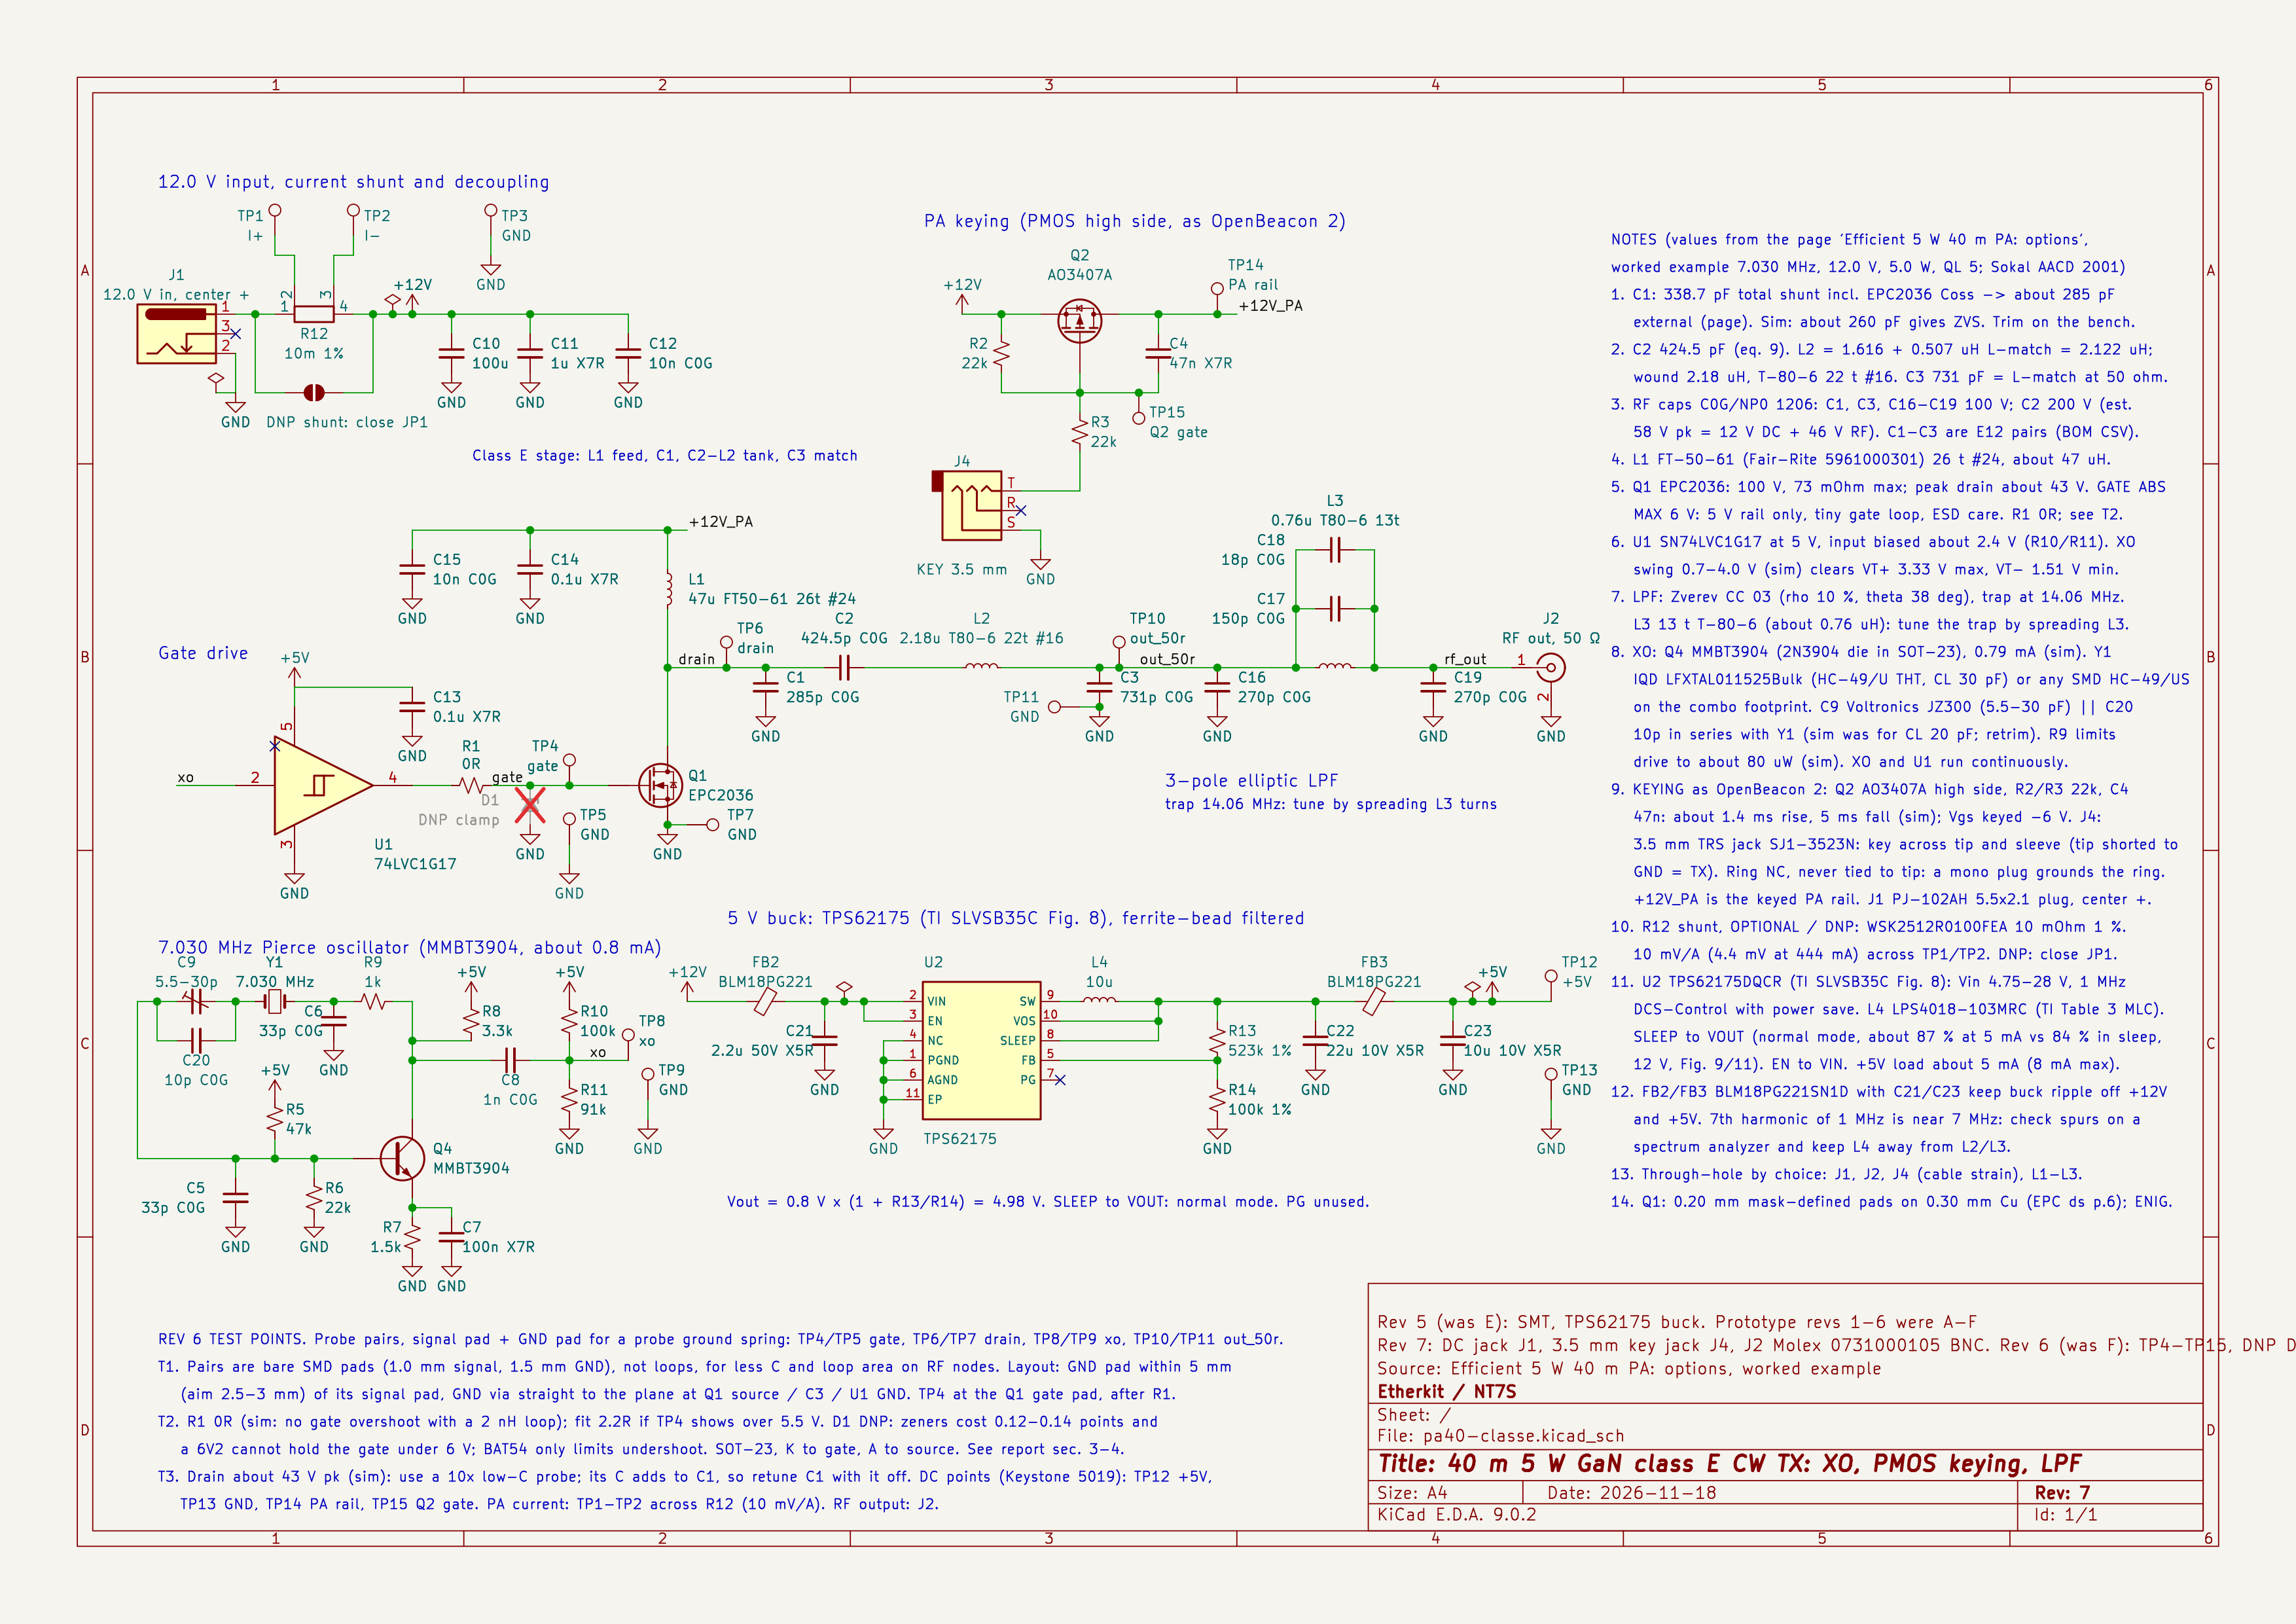
\includegraphics[width=\linewidth,height=0.82\textheight,keepaspectratio]{figures/schematic_rev7.png}
\end{center}
\end{landscape}

\setcounter{biburlnumpenalty}{9000}\setcounter{biburllcpenalty}{7000}\setcounter{biburlucpenalty}{8000}
{\sloppy\printbibliography[heading=bibintoc]}

\end{document}
